\documentclass[acmlarge,review,anonymous]{acmart}\settopmatter{printfolios=true}

\bibliographystyle{ACM-Reference-Format}
\citestyle{acmauthoryear}
\usepackage[english]{babel}
\usepackage{setspace}

\usepackage{paralist} % For inline enumeration
\usepackage{tikz} % For diagrams
\usetikzlibrary{arrows}

\usepackage{isabelle,isabellesym}
\isabellestyle{it}

\hyphenation{App-Jet}

\setcopyright{none} % For review submission

\begin{document}
\title{Formal Verification of Peer-to-Peer Collaborative Editing}
%\author{Victor~B.~F.~Gomes, Martin Kleppmann, Dominic P.~Mulligan,\\Alastair R. Beresford}
%\date{Computer Laboratory, University of Cambridge}

\maketitle

\begin{abstract}
To be completed...
\end{abstract}

%%%%%%%%%%%%%%%%%%%%%%%%%%%%%%%%%%%%%%%%%%%%%%%%%%%%%%%%%%%%%%%%%%%%%%%%%%%%%%%%
% Introduction
%%%%%%%%%%%%%%%%%%%%%%%%%%%%%%%%%%%%%%%%%%%%%%%%%%%%%%%%%%%%%%%%%%%%%%%%%%%%%%%%

\section{Introduction}
\label{sect.introduction}

It is almost a clich{\' e} to say that programming distributed systems is hard. Even the most basic
needs of applications---such as \emph{replication}, that is, maintaining a consistent copy of some
data on several nodes---turn out to be difficult to reliably achieve in the face of unreliable
networks and node failures. In this context, a node can be any computer connected to a network, such
as a server in a datacenter, a laptop, a smartphone, or a self-driving car.

Two instances of the replication problem are
\begin{inparaenum}
\item \emph{collaborative editing}, where the data in question is typically a document (text,
    spreadsheet, graphics, CAD, etc.), and several users need to work on it;
\item \emph{data synchronisation}---for example of calendars, address books, note-taking tools,
    to-do lists, and password managers---which is used when a user owns several devices and wants
    the data accessible on each device.
\end{inparaenum}
In both instances, the system must either enforce an exclusive lock for one node and prevent others
from modifying the data concurrently, or deal with the conflicts that ensue when edits are made
concurrently on different nodes.

Enforcing an exclusive lock implies making the data unavailable for writes when a node is offline,
i.e., when it cannot check whether another node already has the lock. Such unavailability is not
acceptable in many applications, so the latter route of accepting and handling conflicts is widely
used: most calendar, address book, and note-taking apps on smartphones, and popular collaborative
editing applications such as Google Docs/Sheets and Microsoft Office Online, choose to allow
conflicts and have mechanisms for resolving them.

However, despite decades of work in both industry and academia, algorithms for achieving replication
with conflict resolution in distributed systems are still poorly understood. As we document in
Section~\ref{sect.relatedwork}, many published algorithms have been shown to be broken, corrupting
the data they are supposed to replicate. Those that are correct tend to be very subtle and easy to
get wrong.

In this work we advance the state of the art of distributed programming by establishing a framework
for formally verifying the correctness of algorithms for achieving consistency in replication,
conflict resolution, and data synchronisation. We demonstrate, for the first time, machine-checked
proofs of correctness of several replicated data structures. Our framework provides general-purpose
tools for such correctness proofs, allowing other algorithms to be verified more easily in future.

%%%%%

Most deployed systems today address replication problems by relying on a central server that is
trusted to hold the authoritative copy of the data, i.e. by making the distributed system less
distributed. The use of a central server introduces a number of limitations:
\begin{itemize}
\item It limits offline usage: for example, a user cannot synchronise changes between their
    smartphone and laptop via a local wireless connection, but must instead connect both devices to
    the internet. It also rules out a group of users collaborating on a local network disconnected
    from the server, for example in a remote location without reliable internet connectivity.
\item Since the central server holds the authoritative copy of the data, all participants must be
    willing to trust it to a high degree. If the server were compromised by attackers, or subverted
    by a malicious insider, it could tamper with the data or grant access to unauthorised parties.
\item Finally, a central server is a single point of failure that is susceptible to distributed
    denial-of-service (DDoS) attacks, blocking, and censorship. For important services that require
    high availability, the risk of being knocked offline by a DDoS attack might be unacceptable. In
    sensitive situations, such as communication among journalists and dissidents under a repressive
    regime, centralisation of communication is also problematic.
\end{itemize}

Decentralised peer-to-peer systems therefore look attractive in scenarios where reliance on a
central server is impractical or undesirable. Unfortunately, we currently have a poor understanding
of algorithms that enable collaborative editing and data synchronisation in peer-to-peer networks.
In Section~\ref{sect.relatedwork} we highlight several algorithms for peer-to-peer collaboration,
published in peer-reviewed venues, that claimed to work correctly but were subsequently shown to violate
their supposed guarantees. Informal reasoning in this domain has repeatedly produced algorithms that
look plausible, but actually turn out to be flawed.

In this work, we contribute to a better understanding of algorithms for peer-to-peer collaboration
by establishing techniques for formally verifying their correctness. We use Isabelle, a generic
proof assistant tool \cite{DBLP:conf/tphol/WenzelPN08}, to create formal specifications of an
asynchronous network and distributed algorithms executing in such a system. We then use this
framework to produce a machine-checked proof of correctness of one particular algorithm for
peer-to-peer collaboration---the Replicated Growable Array (RGA) of \citet{Roh:2011dw}, an example
of a Conflict-Free Replicated Data Type (CRDT) as introduced by
\citet{Shapiro:2011wy,Shapiro:2011un}.
The algorithm is subtle---\citet{Attiya:2016kh} wrote, ``the reason why RGA actually works has been
a bit of a mystery''---which makes formal verification particularly important.

% TODO say more about our contributions. Can recycle some of the following text, but probably needs
% adapting, as the explanation of CRDTs and OT has been moved to the background section...
%
% To date there has been little formal verification of the correctness of CRDTs, and the
% history of broken OT algorithms highlights the inadequacy of informal reasoning in this domain. In
% this work we contribute to the formal basis of collaborative editing algorithms by using the
% interactive proof assistant Isabelle to develop machine-checked proofs of the
% correctness for CRDTs.
%
% By including a model of the network in our proof, we rule out a larger set of potential errors in
% the algorithm that may result from the interaction of operation properties with assumptions about
% the network. Moreover, our network model and convergence theorems are independent of any particular
% CRDT, so they can be reused for correctness proofs of any other replicated datatype that is based on
% operation commutativity, encompassing a wide range of CRDTs~\cite{Baquero:2014ed}.
%
% Besides presenting the first machine-checked proof of the RGA algorithm, our main contribution in
% this paper is to establish a modular toolkit of proof techniques and building blocks for
% machine-checked correctness proofs of operation-based CRDTs. Our proofs are broken down into modules
% with well-defined properties, allowing modules to be reused for proofs of new datatypes in future.
% By making formal verification easier, we hope to provide a strong foundation for the development of

% the next generation of algorithms for collaborative editing.

% TODO put this in section on high-level proof strategy, and just have a forward reference here?
%Our proof is structured in four modules:
%\begin{inparaenum}
%    \item a general convergence theorem that applies in any system where concurrent operations are
%        commutative;
%    \item a formal model of a network protocol providing reliable, causally-ordered broadcast;
%    \item an implementation of the RGA algorithm, and a proof that well-formed, concurrent insertion
%        and deletion operations commute; and
%    \item a proof that when the RGA algorithm is executed in our network model, all possible
%        executions are well-formed, and thus converge.
%\end{inparaenum}


%%%%%%%%%%%%%%%%%%%%%%%%%%%%%%%%%%%%%%%%%%%%%%%%%%%%%%%%%%%%%%%%%%%%%%%%%%%%%%%%
% Background
%%%%%%%%%%%%%%%%%%%%%%%%%%%%%%%%%%%%%%%%%%%%%%%%%%%%%%%%%%%%%%%%%%%%%%%%%%%%%%%%

\section{Background}
\label{sect.background}

\begin{figure}
\centering
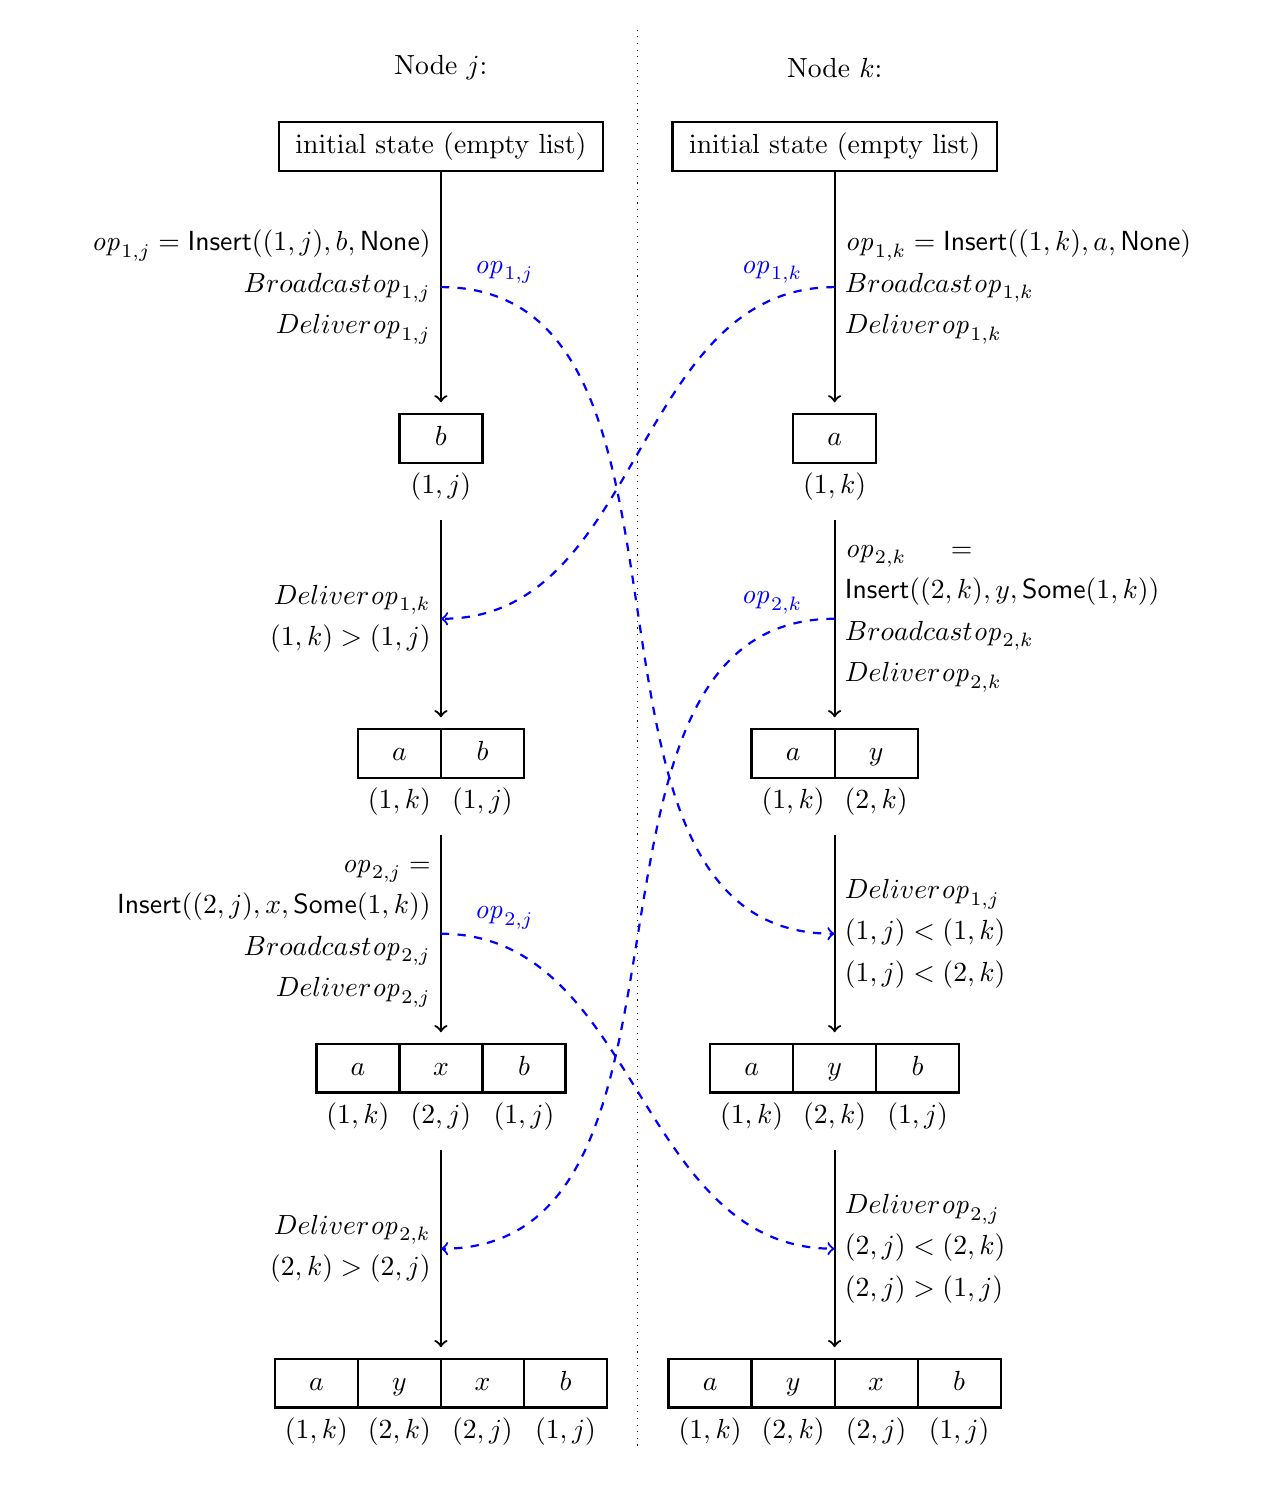
\begin{tikzpicture}[auto,scale=1.0]
\onehalfspacing
\path [draw,dotted] (2.5,-0.5) -- (2.5,17.5);

\tikzstyle{initstate}=[rectangle,draw,inner xsep=6pt,text height=8pt,text depth=3pt]
\tikzstyle{state}=[matrix,column sep={30pt,between origins}]
\tikzstyle{val}=[draw,anchor=base,minimum width=30pt,text height=8pt,text depth=3pt]
\tikzstyle{oid}=[anchor=base]
\tikzstyle{leftevent}=[left,text width=5cm,text ragged left,midway]
\tikzstyle{rightevent}=[right,text width=5cm,text ragged,midway]
\tikzstyle{every path}=[thick,->]

\node (leftR) at (0,17) {Node $j$:};
\node (left1) at (0,16) [initstate] {initial state (empty list)};
\node (left2) at (0,12) [state] {
    \node [val] {$b$};     \\
    \node [oid] {$(1,j)$}; \\
};
\node (left3) at (0,8) [state] {
    \node [val] {$a$};     & \node [val] {$b$};     \\
    \node [oid] {$(1,k)$}; & \node [oid] {$(1,j)$}; \\
};
\node (left4) at (0,4) [state] {
    \node [val] {$a$};     & \node [val] {$x$};     & \node [val] {$b$};     \\
    \node [oid] {$(1,k)$}; & \node [oid] {$(2,j)$}; & \node [oid] {$(1,j)$}; \\
};
\node (left5) at (0,0) [state] {
    \node [val] {$a$};     & \node [val] {$y$};     & \node [val] {$x$};     & \node [val] {$b$};     \\
    \node [oid] {$(1,k)$}; & \node [oid] {$(2,k)$}; & \node [oid] {$(2,j)$}; & \node [oid] {$(1,j)$}; \\
};

\draw (left1) -- (left2) node (send1j) [leftevent] {
    \hfill $\mathit{op}_{1,j} = \mathsf{Insert}((1, j), b, \mathsf{None})$ \\
    \hfill $\text{Broadcast } \mathit{op}_{1,j}$ \\
    \hfill $\text{Deliver } \mathit{op}_{1,j}$ \\
};
\draw (left2) -- (left3) node (recv1k) [leftevent] {
    \hfill $\text{Deliver } \mathit{op}_{1,k}$ \\
    \hfill $(1,k) > (1,j)$ \\
};
\draw (left3) -- (left4) node (send2j) [leftevent] {
    \hfill $\mathit{op}_{2,j} = \mathsf{Insert}((2, j), x, \mathsf{Some}(1,k))$ \\
    \hfill $\text{Broadcast } \mathit{op}_{2,j}$ \\
    \hfill $\text{Deliver } \mathit{op}_{2,j}$ \\
};
\draw (left4) -- (left5) node (recv2k) [leftevent] {
    \hfill $\text{Deliver } \mathit{op}_{2,k}$ \\
    \hfill $(2,k) > (2,j)$ \\
};

\node (rightR) at (5,17) {Node $k$:};
\node (right1) at (5,16) [initstate] {initial state (empty list)};
\node (right2) at (5,12) [state] {
    \node [val] {$a$};     \\
    \node [oid] {$(1,k)$}; \\
};
\node (right3) at (5,8) [state] {
    \node [val] {$a$};     & \node [val] {$y$};     \\
    \node [oid] {$(1,k)$}; & \node [oid] {$(2,k)$}; \\
};
\node (right4) at (5,4) [state] {
    \node [val] {$a$};     & \node [val] {$y$};     & \node [val] {$b$};     \\
    \node [oid] {$(1,k)$}; & \node [oid] {$(2,k)$}; & \node [oid] {$(1,j)$}; \\
};
\node (right5) at (5,0) [state] {
    \node [val] {$a$};     & \node [val] {$y$};     & \node [val] {$x$};     & \node [val] {$b$};     \\
    \node [oid] {$(1,k)$}; & \node [oid] {$(2,k)$}; & \node [oid] {$(2,j)$}; & \node [oid] {$(1,j)$}; \\
};

\draw (right1) -- (right2) node (send1k) [rightevent] {
    $\mathit{op}_{1,k} = \mathsf{Insert}((1, k), a, \mathsf{None})$ \\
    $\text{Broadcast } \mathit{op}_{1,k}$ \\
    $\text{Deliver } \mathit{op}_{1,k}$ \\
};
\draw (right2) -- (right3) node (send2k) [rightevent] {
    $\mathit{op}_{2,k} = \mathsf{Insert}((2, k), y, \mathsf{Some}(1, k))$ \\
    $\text{Broadcast } \mathit{op}_{2,k}$ \\
    $\text{Deliver } \mathit{op}_{2,k}$ \\
};
\draw (right3) -- (right4) node (recv1j) [rightevent] {
    $\text{Deliver } \mathit{op}_{1,j}$ \\
    $(1,j) < (1,k)$ \\
    $(1,j) < (2,k)$ \\
};
\draw (right4) -- (right5) node (recv2j) [rightevent] {
    $\text{Deliver } \mathit{op}_{2,j}$ \\
    $(2,j) < (2,k)$ \\
    $(2,j) > (1,j)$ \\
};

\begin{scope}[dashed,blue]
    \tikzstyle{every node}=[text centered]
    \draw (send1j.east) to [out=0,in=180] (recv1j.west);
    \draw (send2j.east) to [out=0,in=180] (recv2j.west);
    \draw (send1k.west) to [out=180,in=0] (recv1k.east);
    \draw (send2k.west) to [out=180,in=0] (recv2k.east);
    \node at (0.8,14.4) {$\mathit{op}_{1,j}$};
    \node at (0.8, 6.2) {$\mathit{op}_{2,j}$};
    \node at (4.2,14.4) {$\mathit{op}_{1,k}$};
    \node at (4.2,10.2) {$\mathit{op}_{2,k}$};
\end{scope}
\end{tikzpicture}

\caption{RGA example}\label{fig.two-lists}
\end{figure}



\subsection{An overview of Isabelle}
\label{subsect.an.overview.of.isabelle}

All of our proofs are checked with the Isabelle/HOL proof assistant~\cite{DBLP:conf/tphol/WenzelPN08}, which we now briefly introduce so that the reader can easily follow our work.
A more detailed introduction is provided by standard tutorial material~\cite{DBLP:books/sp/NipkowK14}.

Isabelle/HOL is a logic with a strict, polymorphic type system resembling that of mainstream functional programming languages.
\emph{Function types} are written $\tau_1 \Rightarrow \tau_2$, and are inhabited by \emph{total} functions, mapping elements of $\tau_1$ to elements of $\tau_2$.
We write $\tau_1 \times \tau_2$ for the \emph{product type} of $\tau_1$ and $\tau_2$, inhabited by pairs of elements of type $\tau_1$ and $\tau_2$, respectively.
In a similar fashion to Standard ML and OCaml, but differing from Haskell, \emph{type operators} are applied to arguments in reverse order, and therefore write $\tau\ \isa{list}$ and $\tau\ \isa{set}$ for the type of lists of elements of type $\tau$, and the type of mathematical (i.e. potentially infinite) sets of type $\tau$, respectively.
Type variable are written in lowercase, and preceded with a prime: ${\isacharprime}a \Rightarrow {\isacharprime}a$ denotes the type of a polymorphic identity function, for example.
\emph{Tagged union} types are introduced with the $\isacommand{datatype}$ keyword, with constructors of these types written with an initial upper case letter.

In Isabelle/HOL's term language we write $\isa{t} \isa{::} \tau$ for a \emph{type ascription}, constraining the type of the term $\isa{t}$ to the type $\tau$.
We write $\lambda{x}. t$ for an anonymous function mapping an argument $\isa{x}$ to $\isa{t(x)}$, and write the application of term $\isa{t}$ with function type to an argument $\isa{u}$ as $\isa{t\ u}$, as usual.
Terms of list type are introduced using one of two constructors: $\isa{[]}$, or `nil', standing for the empty list, and infix $\isa{\#}$, or `cons', which prepends an element to an existing list.
We use $[t_1, \ldots, t_n]$ as syntactic sugar for a list literal, which is desugared into a series of cons applications.
We write $\{\}$ for the empty set, and use usual mathematical notation for set union, disjunction, membership tests, and so on: $\isa{t} \cup \isa{u}$, $\isa{t} \cap \isa{u}$, and $\isa{x} \in \isa{t}$.

Terms with type $\isa{bool}$ are called \emph{formulae}, writing $\isa{True}$ and $\isa{False}$ for the logical truthity and falsity constants, respectively.
We write $\isa{t} \longrightarrow \isa{u}$, $\isa{t} \wedge \isa{u}$, and $\isa{t} \vee \isa{u}$ for material implication, conjunction, and disjunction, respectively, between formulae, and write $\neg t$ for the negation of a formula.
Isabelle/HOL's equality constant is polymorphic: we write $t = u$ for an assertion of equality between two terms of the same type.
We write $\forall{x}.t$ and $\exists{x}.t$ for universal and existential quantification---and write $\forall{x{\in}t}.u$ and $\exists{x{\in}t}.u$ for their bounded forms, restricted to members of a set $\isa{t}$.
An alternative implication arrow $\isa{t} \Longrightarrow \isa{u}$ may sometimes be used, and is in fact required by Isabelle in certain contexts---an artefact of Isabelle's status as a logical framework.
This arrow can safely be read as a standard implication arrow with little loss of understanding.

New non-recursive definitions are entered into Isabelle's global context via the $\mathbf{definition}$ keyword.
Recursive functions are entered via the $\mathbf{fun}$ keyword, with functions being defined piecewise by pattern matching on inputs with a series of equations.
All function are total, and therefore recursive functions must be provably terminating, in that they recurse on arguments that are `smaller' with respect to a well-founded relation.
All termination proofs in this work are generated automatically by Isabelle itself.

Inductive relations are introduced with the $\mathbf{inductive}$ keyword.
An inductive relation definition of the form
\\
\begin{isabellebody}
\ \ \ \ \ \ \ \ \isacommand{inductive} foo\ {\isacharcolon}{\isacharcolon}\ {\isachardoublequoteopen}nat\ list\ {\isasymRightarrow}\ bool{\isachardoublequoteclose}\ \isakeyword{where}\isanewline
\ \ \ \ \ \ \ \ \ \ {\isachardoublequoteopen}foo\ {\isacharbrackleft}{\isacharbrackright}{\isachardoublequoteclose}\ {\isacharbar}\isanewline
\ \ \ \ \ \ \ \ \ \ {\isachardoublequoteopen}{\isasymlbrakk}\ foo\ xs\ {\isasymrbrakk}\ {\isasymLongrightarrow}\ foo {\isacharparenleft}5\#xs{\isacharparenright}{\isachardoublequoteclose}
\end{isabellebody}
\vspace{\baselineskip}
\noindent
introduces a new constant $\isa{foo}$ of type $\isa{nat list} \Rightarrow \isa{bool}$.
The two clauses in the body of the definition enumerate the conditions under which $\isa{foo}\ \isa{xs}$ is true, for arbitrary $\isa{xs}$.
The definition above states that $\isa{foo}$ is true at the empty list, or given a proof that $\isa{foo}\ \isa{xs}$ is true for some $\isa{xs}$, then $\isa{foo}\ (5\#\isa{xs})$ is true, also.
Further, $\isa{foo}\ \isa{xs}$ is true in no other circumstances---$\isa{foo}$ is the \emph{smallest} relation closed under the rules defining it.
In short, the clauses defining $\isa{foo}$ above state that $\isa{foo}\ \isa{xs}$ holds exactly in the case where $\isa{xs}$ is a (potentially empty) list containing only repeated copies of the natural number $5$.

Lemmas, theorems, and corollaries can be asserted using the $\isacommand{lemma}$, $\isacommand{theorem}$, and $\isacommand{corollary}$ keywords, respectively.
There is no semantic difference between these keywords in Isabelle.
A theorem statement of the form
\\
\begin{isabellebody}
\ \ \ \ \ \ \ \ \isacommand{theorem} goo{\isacharcolon}\isanewline
\ \ \ \ \ \ \ \ \ \ \isakeyword{assumes}\ foo\ xs \isakeyword{and}\ foo\ ys \isanewline
\ \ \ \ \ \ \ \ \ \ \isakeyword{shows}\ foo (xs \isacharat ys)
\end{isabellebody}
\vspace{\baselineskip}
\noindent
produces a proof obligation, wherein the user is tasked with proving $\isa{foo} (xs \isacharat ys)$ under the two assumptions $\isa{foo}\ xs$ and $\isa{foo}\ ys$, where $xs \isacharat ys$ denotes the appending of two lists $\isa{xs}$ and $\isa{ys}$.
An optional name, here $\isa{goo}$, is assigned to the theorem, so that it may be referenced in later proofs.

Lastly, we use \emph{locales}---or local theory environments~\cite{DBLP:conf/tphol/KammullerWP99,DBLP:conf/types/HaftmannW08}---extensively throughout our development to structure the proof.
A declaration of the form
\\
\begin{isabellebody}
\ \ \ \ \ \ \ \ \isacommand{locale} hoo = \isanewline
\ \ \ \ \ \ \ \ \ \ \isakeyword{fixes}\ f\ {\isacharcolon}{\isacharcolon}\ {\isachardoublequoteopen}{\isacharprime}a\ {\isasymRightarrow}\ {\isacharprime}a{\isachardoublequoteclose}\isanewline
\ \ \ \ \ \ \ \ \ \ \isakeyword{assumes} {\isachardoublequoteopen}f\ x = x{\isachardoublequoteclose}
\end{isabellebody}
\vspace{\baselineskip}
\noindent
introduces a local theory, with a fixed, typed constant $\isa{f}$, and an associated law that states that $\isa{f}$ is the identity function.
Functions and constants may now be defined, and theorems conjectured and proved, within the context of the $\isa{hoo}$ theory.
This is indicated syntactically by writing $(\isacommand{in}\ hoo)$ before the name of the constant being defined, or the theorem being conjectured, at the point of definition or conjecture.
Any function, constant, or theorem, marked in this way may make reference to $\isa{f}$, or the fact that $\isa{f}\ \isa{x} = \isa{x}$ for all $\isa{x}$.
\emph{Interpreting} a local theory---such as $\isa{hoo}$ above---involves providing a concrete implementation of $\isa{f}$ coupled with a proof that the concrete implementation satisfies the associated law.
Once interpreted, all functions, definitions, and theorems made within the $\isa{hoo}$ local theory become available to use for that concrete implementation.


%%%%%%%%%%%%%%%%%%%%%%%%%%%%%%%%%%%%%%%%%%%%%%%%%%%%%%%%%%%%%%%%%%%%%%%%%%%%%%%%
% Related Work
%%%%%%%%%%%%%%%%%%%%%%%%%%%%%%%%%%%%%%%%%%%%%%%%%%%%%%%%%%%%%%%%%%%%%%%%%%%%%%%%

\section{Related Work}\label{sect.relatedwork}

In a system where different replicas may concurrently perform updates without coordinating with each
other, strong eventual consistency (SEC, see Section~\ref{sect.eventual.consistency}) requires a
conflict resolution algorithm to reconcile concurrent updates. In some cases, a trivial algorithm is
used, for example:

\begin{description}
\item[User-defined conflict resolution:] Some systems store all conflicting versions of the data,
and either leave it for manual resolution by a user, or invoke a user-defined merge function.
However, manual resolution is an unacceptable burden for the user in many applications, and defining
merge functions in application code is error-prone; for example, \citet{DeCandia:2007ui} describe a
shopping cart anomaly at Amazon that arose due to poor conflict resolution.

\item[Last write wins (LWW):] Each version of the data structure is assigned a unique timestamp.
When there is a conflict, the system picks the version with the highest timestamp and discards other
versions. Although LWW achieves convergence, it does so at the cost of losing user input, which is
often unacceptable.
\end{description}

However, there are also algorithms that achieve convergence automatically, without discarding
updates. In Sections~\ref{sect.related.crdts} and~\ref{sect.related.ot} we summarise two main lines
of work, CRDTs and OT, which have the same fundamental goal of conflict resolution and convergence,
but which take different approaches towards achieving it.

\subsection{Conflict-Free Replicated Data Types (CRDTs)}\label{sect.related.crdts}

Some operations, such as addition of numbers, are naturally commutative. Thus, if the replicated
data structure is a number whose value can only be incremented or decremented (a counter),
convergence can be achieved by applying the increment and decrement operations in any order at each
replica.

\emph{Conflict-free replicated data types} (CRDTs) generalise this idea to other data structures and
operations. For example, an ordered list (sequence) of values can be modified by inserting or
deleting elements at specified positions, and a map (dictionary) datatype can be modified by setting
the value associated with a key or deleting a key-value pair from the map. In a CRDT, those
modification operations are constructed to be commutative by attaching additional metadata to the
data structure.

To propagate changes between replicas, a CRDT either captures every update as an operation and
broadcasts it to other replicas (an \emph{operation-based} CRDT), or periodically broadcasts its
entire replica state (a \emph{state-based} CRDT). Operation-based CRDTs require operations to be
commutative; state-based CRDTs require a merge function over a join-semilattice, allowing two states
to be combined such that the result reflects changes made in both replicas. The two models have
different performance characteristics, but equivalent expressivity
\cite{Shapiro:2011wy,Shapiro:2011un}.

Many common abstract datatypes have been formulated as CRDTs, including
registers \cite{Shapiro:2011wy,Shapiro:2011un}, counters, maps \cite{Baquero:2016iv},
sets \cite{Bieniusa:2012wu,Bieniusa:2012gt}, XML \cite{Martin:2010ih},
and JSON trees \cite{Kleppmann:2016ve}. For ordered lists, several algorithms have been defined:
RGA \cite{Roh:2011dw}, Treedoc \cite{Preguica:2009fz}, WOOT \cite{Oster:2006wj},
Logoot \cite{Weiss:2010hx}, and LSEQ \cite{Nedelec:2013ky,Nedelec:2016eo}.
State-based CRDTs have been deployed commercially in the Riak database \cite{Brown:2014hs}.
Cloud types \cite{Burckhardt:2012jy} have similarities to CRDTs, using a relational data model.

In this work we formally verify three representative operation-based CRDTs: a counter
\cite{Shapiro:2011wy}, an OR-Set \cite{Bieniusa:2012gt}, and the RGA algorithm for ordered lists
\cite{Roh:2011dw}. While the counter and set are quite straightforward, RGA is subtle; we first
describe it informally in Section~\ref{sect.rga.background}, before showing how to formally prove
its convergence.


\subsection{Operational Transformation (OT)}\label{sect.related.ot}

Another family of algorithms for achieving convergence of replicas uses the \emph{operational
transformation} (OT) approach. They are designed for collaborative editing, that is, multiple users
concurrently modifying a document on their local device, and propagating updates asynchronously to
other users' devices. The replicated data structure is most commonly assumed to be a text document,
represented as an ordered list of characters that may be modified by inserting or deleting
characters at arbitrary positions in the string. OT algorithms for ordered lists include
dOPT \cite{Ellis:1989ue}, Jupiter \cite{Nichols:1995fd}, adOPTed \cite{Ressel:1996wx},
GOT \cite{Sun:1998un}, GOTO \cite{Sun:1998vf}, SOCT2 \cite{Suleiman:1997gl,Suleiman:1998eu},
SOCT3/4 \cite{Vidot:2000ch}, IMOR \cite{Imine:2003ks}, SDT \cite{Li:2004er,Li:2008hw}, and
TTF \cite{Oster:2006tr}.  The approach has also been generalised to other data structures such as
XML trees \cite{Ignat:2003jy,Davis:2002iv,Jungnickel:2015ua} and vector graphics documents
\cite{Sun:2002jb}.

Unlike CRDTs, in which update operations are commutative by definition, OT allows non-commutative
operations. Instead, OT relies on \emph{transforming} concurrent operations, allowing them to be
reordered on different nodes while ensuring a convergent outcome.

The required properties of this transformation function depend on assumptions about the network.
Many OT algorithms assume that operations are sequenced through a central server and delivered to
all clients in the same order. This design was originally pioneered by the Jupiter system
\cite{Nichols:1995fd} and is now used by all widely-deployed OT-based collaboration systems,
including Google Docs \cite{DayRichter:2010tt}, Microsoft Word Online, Etherpad
\cite{Etherpad:2011um}, Apache (formerly Google) Wave \cite{Wang:2015vo}, and Novell Vibe
\cite{Spiewak:2010vw}. With a central server, each client only needs to reorder its operations with
respect to the server's operation sequence, which simplifies the transformation.

On the other hand, as discussed in Section~\ref{sect.background.networks}, total order broadcast is
too restrictive for many peer-to-peer systems. Without total order broadcast, OT algorithms must
tolerate a higher degree of concurrency. Although a number of OT algorithms were purported to
guarantee convergence in peer-to-peer networks, many of them were later proved to be incorrect, as
discussed in the next section.

\subsection{Formal Verification}\label{sect.related.verification}

Even though a data structure such as an ordered list may seem as though it ought to be simple, the
history of algorithms for achieving convergence in a distributed setting has been fraught with
difficulty. Informal reasoning has repeatedly produced approaches that fail to converge in certain
scenarios, and even several formal ``proofs'' later turned out to be false.

For OT, the properties that the transformation function must satisfy were first formalised by
\citet{Ressel:1996wx}. These properties are known as $\mathit{TP}_1$ and $\mathit{TP}_2$; systems
with a central server or total order broadcast need only satisfy $\mathit{TP}_1$, whereas
decentralised systems must satisfy both properties in order to ensure convergence. While
$\mathit{TP}_1$ has proved to be readily achievable in practice, and all the aforementioned
widely-deployed OT systems rely on it, the $\mathit{TP}_2$ property has been a significant source of
problems.

The original peer-reviewed publications of dOPT, adOPTed, IMOR, SOCT2, and SDT all claimed that
their transformation functions satisfied $\mathit{TP}_2$, but those claims were subsequently shown
to be false by giving counter-examples \cite{Imine:2003ks,Imine:2006kn,Oster:2005vi}. In the case of
dOPT and adOPTed, the $\mathit{TP}_2$ claim had originally been asserted without proof. In the case
of SOCT2 and SDT, there were hand-written ``proofs'' that later turned out to be incorrect. For IMOR
and SOCT2, there had even been machine-checked ``proofs'' \cite{Imine:2003ks}, but
\citet{Oster:2005vi} showed that they also were invalid because they made incorrect assumptions.

\citet{Randolph:2015gj} have even shown that in the classic formulation of OT it is impossible to
achieve $\mathit{TP}_2$. To our knowledge, TTF is at present the only $\mathit{TP}_2$-claiming OT
algorithm for which no counter-example is known, and it circumvents the impossibility result of
\citet{Randolph:2015gj} by using a different formulation of the transformation
\cite{Oster:2006tr,Levien:2016wz}.

Formal proofs of the $\mathit{TP}_1$ property have been more successful: \citet{Sinchuk:2016cf} and
\citet{Jungnickel:2015ua} verify transformation functions for trees, using Coq and Isabelle/HOL
respectively. For CRDTs, the only machine-checked verification of which we are aware is an Isabelle
formalisation of state-based sets, registers, and counters by \citet{Zeller:2014fl}; this work does
not consider any ordered list datatypes or any operation-based CRDTs.

The convergence of the RGA CRDT for ordered lists, which we study in this paper, has previously been
demonstrated in handwritten proofs \cite{Attiya:2016kh,Kleppmann:2016ve,Roh:2009ws}. Although we
have no reason to doubt the correctness of those proofs, the historic experience with
$\mathit{TP}_2$ makes us wary of claims whose assumptions and reasoning process have not been
checked rigorously. Other authors have also pointed out that handwritten proofs are laborious and
difficult to check by hand \cite{Li:2008hw,Li:2005jq}.

To our knowledge, our work is the first mechanised proof of operation-based CRDTs in general, and of
any ordered list CRDT in particular. As \citet{Oster:2005vi} have demonstrated, machine-checked
proofs are not immune to errors that are due to false assumptions. To avoid this trap, we prove not
only the commutativity of operations (which is subject to certain assumptions), but also that those
assumptions are guaranteed to hold in all executions of our network model. The network model in turn
is specified by a small set of axioms that are not specific to any particular CRDT, and whose
correctness can be robustly defended (see Section~\ref{sect.network}).

\citet{Burckhardt:2014ft} present a similar framework for reasoning about replicated datatypes, but
do not support mechanised proofs at present.


\section{The Replicated Growable Array (RGA)}\label{sect.rga.background}

In order to develop an intuition for the problems that arise in concurrent editing systems, we now
discuss an example execution of the \emph{Replicated Growable Array} (RGA) algorithm, a CRDT for
ordered lists that supports insertion and deletion of arbitrary elements. RGA was developed by
\citet{Roh:2011dw}, although our presentation of the algorithm more closely follows that of
\citet{Shapiro:2011wy}. We start with the informal example illustrated in
Figure~\ref{fig.two-lists}, and leave the formal specification of RGA until Section~\ref{sect.rga}.

In this paper we
choose to analyze RGA because it is a subtle algorithm that benefits from formal verification
\cite{Attiya:2016kh}, because it has been shown to have good performance \cite{Mehdi:2011ke}, and
because it has been generalised to more general data structures such as JSON
\cite{Kleppmann:2016ve}, enabling our work to be extended towards those more general data structures
in future.

RGA is based on the idea of assigning a unique identifier (ID) to each list element, and using a
total ordering relation over IDs to ensure convergence. When the list is modified through insertion
and deletion operations, the ID of an existing element is used to identify the position in the list
being modified. Using an ID has the advantage that it continues to refer to the same list element
regardless of any concurrent operations, whereas list indexes change (for example, inserting a list
element at the beginning increases the index of every subsequent list element by 1).

We use the logical timestamps defined by \citet{Lamport:1978jq} as IDs.

% In this setting, causally ordered delivery is the strongest
% guarantee that can reliably be provided \cite{Attiya:2015dm}.

% \subsubsection{Causal Ordering}
\subsection{Causality and the Happens-Before Relation}\label{sect.causality}

Most operation-based CRDTs and OT algorithms require that operations are processed in an order that
is \emph{consistent with causality}. Informally, this means that later operations may depend on
earlier operations; for example, the deletion of a list element depends on the prior insertion of
that list element. It makes no sense for a replica to apply the deletion before it applies the
insertion, because that would mean deleting an element that does not yet exist at that time.

In this context, referring to operations as ``earlier'' or ``later'' does not mean comparing the
physical time in UTC at which those operations occurred; relying on physical time is often
problematic in distributed systems \cite{Sheehy:2015jm}. Instead we say that an operation
$\mathit{op}_1$ \emph{happens before} another operation $\mathit{op}_2$ if the node that generated
$\mathit{op}_2$ ``knew about'' $\mathit{op}_1$ at the time $\mathit{op}_2$ was generated (i.e., if
$\mathit{op}_1$ had already been applied at that time). If the node knew about $\mathit{op}_1$, then
$\mathit{op}_2$ may somehow be caused by it, but if it didn't know about $\mathit{op}_1$, we can be
certain that $\mathit{op}_2$ does not depend on it.

We write $\mathit{op}_1 \prec \mathit{op}_2$ if $\mathit{op}_1$ happens before $\mathit{op}_2$. (In
the distributed systems literature, the happens-before relation is usually written
$\mathit{op}_1 \longrightarrow \mathit{op}_2$, but we reserve the arrow to refer to logical
implication.) Following the definition by \citet{Lamport:1978jq}, we say that
$\mathit{op}_1 \prec \mathit{op}_2$ if any of the following is true:

\begin{itemize}
\item $\mathit{op}_1$ and $\mathit{op}_2$ were generated by the same node, and that node generated
    $\mathit{op}_1$ before it generated $\mathit{op}_2$.
\item The node that generated $\mathit{op}_2$ had received and applied $\mathit{op}_1$ before it
    generated $\mathit{op}_2$.
\item There exists some operation $\mathit{op}_3$ such that
    $\mathit{op}_1 \prec \mathit{op}_3$ and $\mathit{op}_3 \prec \mathit{op}_2$.
\end{itemize}

\begin{figure}
\centering
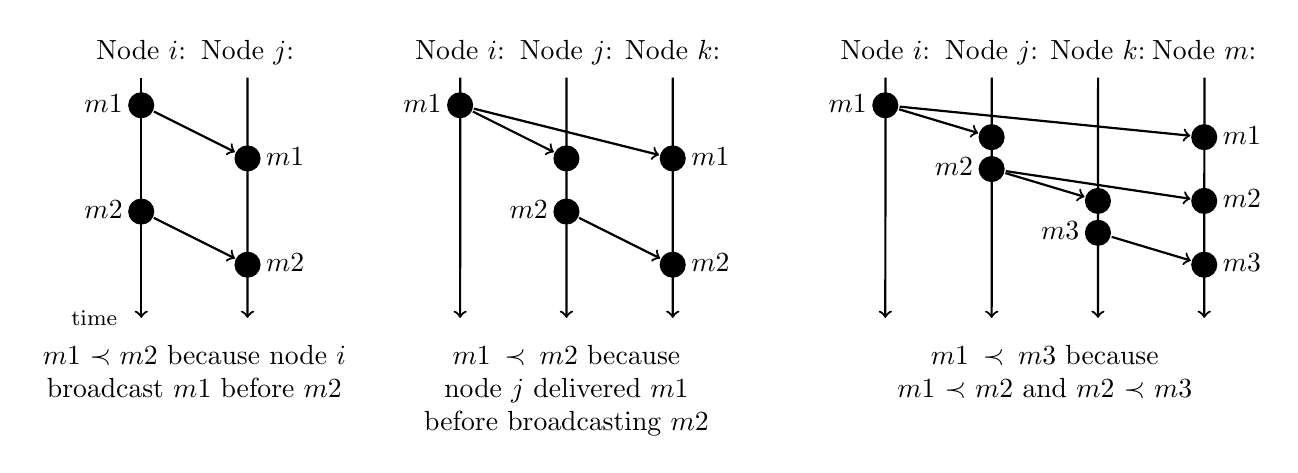
\begin{tikzpicture}[auto,scale=1.35]

\tikzstyle{event}=[circle,fill,minimum size=2pt]
\tikzstyle{label}=[text height=8pt,text depth=3pt]
\tikzstyle{leftlabel}=[label,left=3pt]
\tikzstyle{rightlabel}=[label,right=3pt]
\tikzstyle{every path}=[thick,->]
\tikzstyle{caption}=[text width=4cm,text centered,text height=8pt,below=5pt]

\node [label] (i1name) at (0,2.5) {Node $i$:};
\node [label] (j1name) at (1,2.5) {Node $j$:};
\node [event] (op1send) at (0,2.0) {};
\node [event] (op1recv) at (1,1.5) {};
\node [event] (op2send) at (0,1.0) {};
\node [event] (op2recv) at (1,0.5) {};
\node [leftlabel]  at (0,2.0) {$\isa{m1}$};
\node [rightlabel] at (1,1.5) {$\isa{m1}$};
\node [leftlabel]  at (0,1.0) {$\isa{m2}$};
\node [rightlabel] at (1,0.5) {$\isa{m2}$};
\draw (i1name) -- (0,0) node [left=5pt,at end] {\footnotesize time};
\draw (j1name) -- (1,0);
\draw (op1send) -- (op1recv);
\draw (op2send) -- (op2recv);
\node [caption] at (0.5,0) {
    $\isa{m1} \prec \isa{m2}$
    because node $i$ broadcast $\isa{m1}$ before $\isa{m2}$
};

\node [label] (i2name) at (3,2.5) {Node $i$:};
\node [label] (j2name) at (4,2.5) {Node $j$:};
\node [label] (k2name) at (5,2.5) {Node $k$:};
\node [event] (op3send) at (3,2.0) {};
\node [event] (op3recj) at (4,1.5) {};
\node [event] (op3reck) at (5,1.5) {};
\node [event] (op4send) at (4,1.0) {};
\node [event] (op4reck) at (5,0.5) {};
\node [leftlabel]  at (3,2.0) {$\isa{m1}$};
\node [rightlabel] at (5,1.5) {$\isa{m1}$};
\node [leftlabel]  at (4,1.0) {$\isa{m2}$};
\node [rightlabel] at (5,0.5) {$\isa{m2}$};
\draw (i2name) -- (3,0);
\draw (j2name) -- (4,0);
\draw (k2name) -- (5,0);
\draw (op3send) -- (op3recj);
\draw (op3send) -- (op3reck);
\draw (op4send) -- (op4reck);
\node [caption] at (4.0,0) {
    $\isa{m1} \prec \isa{m2}$
    because node $j$ delivered $\isa{m1}$ before broadcasting $\isa{m2}$
};

\node [label] (i3name) at  (7,2.5) {Node $i$:};
\node [label] (j3name) at  (8,2.5) {Node $j$:};
\node [label] (k3name) at  (9,2.5) {Node $k$:};
\node [label] (m3name) at (10,2.5) {Node $m$:};
\node [event] (op5send) at  (7,2.0) {};
\node [event] (op5recj) at  (8,1.7) {};
\node [event] (op5recm) at (10,1.7) {};
\node [event] (op6send) at  (8,1.4) {};
\node [event] (op6reck) at  (9,1.1) {};
\node [event] (op6recm) at (10,1.1) {};
\node [event] (op7send) at  (9,0.8) {};
\node [event] (op7recm) at (10,0.5) {};
\node [leftlabel]  at  (7,2.0) {$\isa{m1}$};
\node [rightlabel] at (10,1.7) {$\isa{m1}$};
\node [leftlabel]  at  (8,1.4) {$\isa{m2}$};
\node [rightlabel] at (10,1.1) {$\isa{m2}$};
\node [leftlabel]  at  (9,0.8) {$\isa{m3}$};
\node [rightlabel] at (10,0.5) {$\isa{m3}$};
\draw (i3name) -- (7,0);
\draw (j3name) -- (8,0);
\draw (k3name) -- (9,0);
\draw (m3name) -- (10,0);
\draw (op5send) -- (op5recj);
\draw (op5send) -- (op5recm);
\draw (op6send) -- (op6reck);
\draw (op6send) -- (op6recm);
\draw (op7send) -- (op7recm);
\node [caption] at (8.5,0) {
    $\isa{m1} \prec \isa{m3}$ because
    $\isa{m1} \prec \isa{m2}$ and
    $\isa{m2} \prec \isa{m3}$
};

\end{tikzpicture}

\caption{Illustrating the happens-before relation}\label{fig.happens-before}
\end{figure}

Figure~\ref{fig.happens-before} illustrates these three cases, and the formalisation of this
definition appears in Section~\ref{sect.network}.

In practice, the happens-before relationship can be captured using vector timestamps
\cite{Schwarz:1994gl,Fidge:1988tv,Raynal:1996jl}, which are used to implement protocols for causally
ordered delivery \cite{Cachin:2011wt}. As these protocols are widely known and well understood, we
leave them out of scope for this paper.


% Total order broadcast ensures that when nodes broadcast a set of messages to other nodes on the
% network, they are delivered in the same order to all recipients. By contrast, causal ordering is a
% weaker guarantee that allows greater concurrency and thus greater nondeterminism in the network.
% However, it has the advantage that it makes no assumptions about the number of nodes that are
% online.

% TODO happens-before


% There are two families of algorithms for collaborative editing: \emph{operational transformation}
% (OT)~\cite{Ellis:1989ue,Ressel:1996wx,Oster:2006tr,Sun:1998vf,Sun:1998un,Suleiman:1998eu,Nichols:1995fd}
% and \emph{conflict-free replicated datatypes}
% (CRDTs)~\cite{Shapiro:2011wy,Roh:2011dw,Preguica:2009fz,Oster:2006wj,Weiss:2010hx,Nedelec:2013ky,Kleppmann:2016ve}.
% Both allow a document to be modified concurrently on different replicas, with changes applied
% immediately to the local copy, while asynchronously propagating changes to other replicas. The
% goal of these algorithms is to ensure that for all concurrent executions, the replicas converge
% toward the same state without any edits being lost, a property known as \emph{strong eventual
% consistency}~\cite{Shapiro:2011un}.


% CRDTs are a more recent development~\cite{Shapiro:2011un}. While OT is based on transforming
% non-commutative operations so that they have the same effect when reordered, CRDTs define operations
% in a way that makes them commutative by design, making them more amenable to peer-to-peer settings
% in which each node may apply edits in a different order. CRDTs also have attractive performance
% characteristics~\cite{Mehdi:2011ke}.

% TODO Various decentralised algorithms have been proposed and all but one (Oster 2006) have
% subsequently been shown to be incorrect.

\begin{figure}
\centering
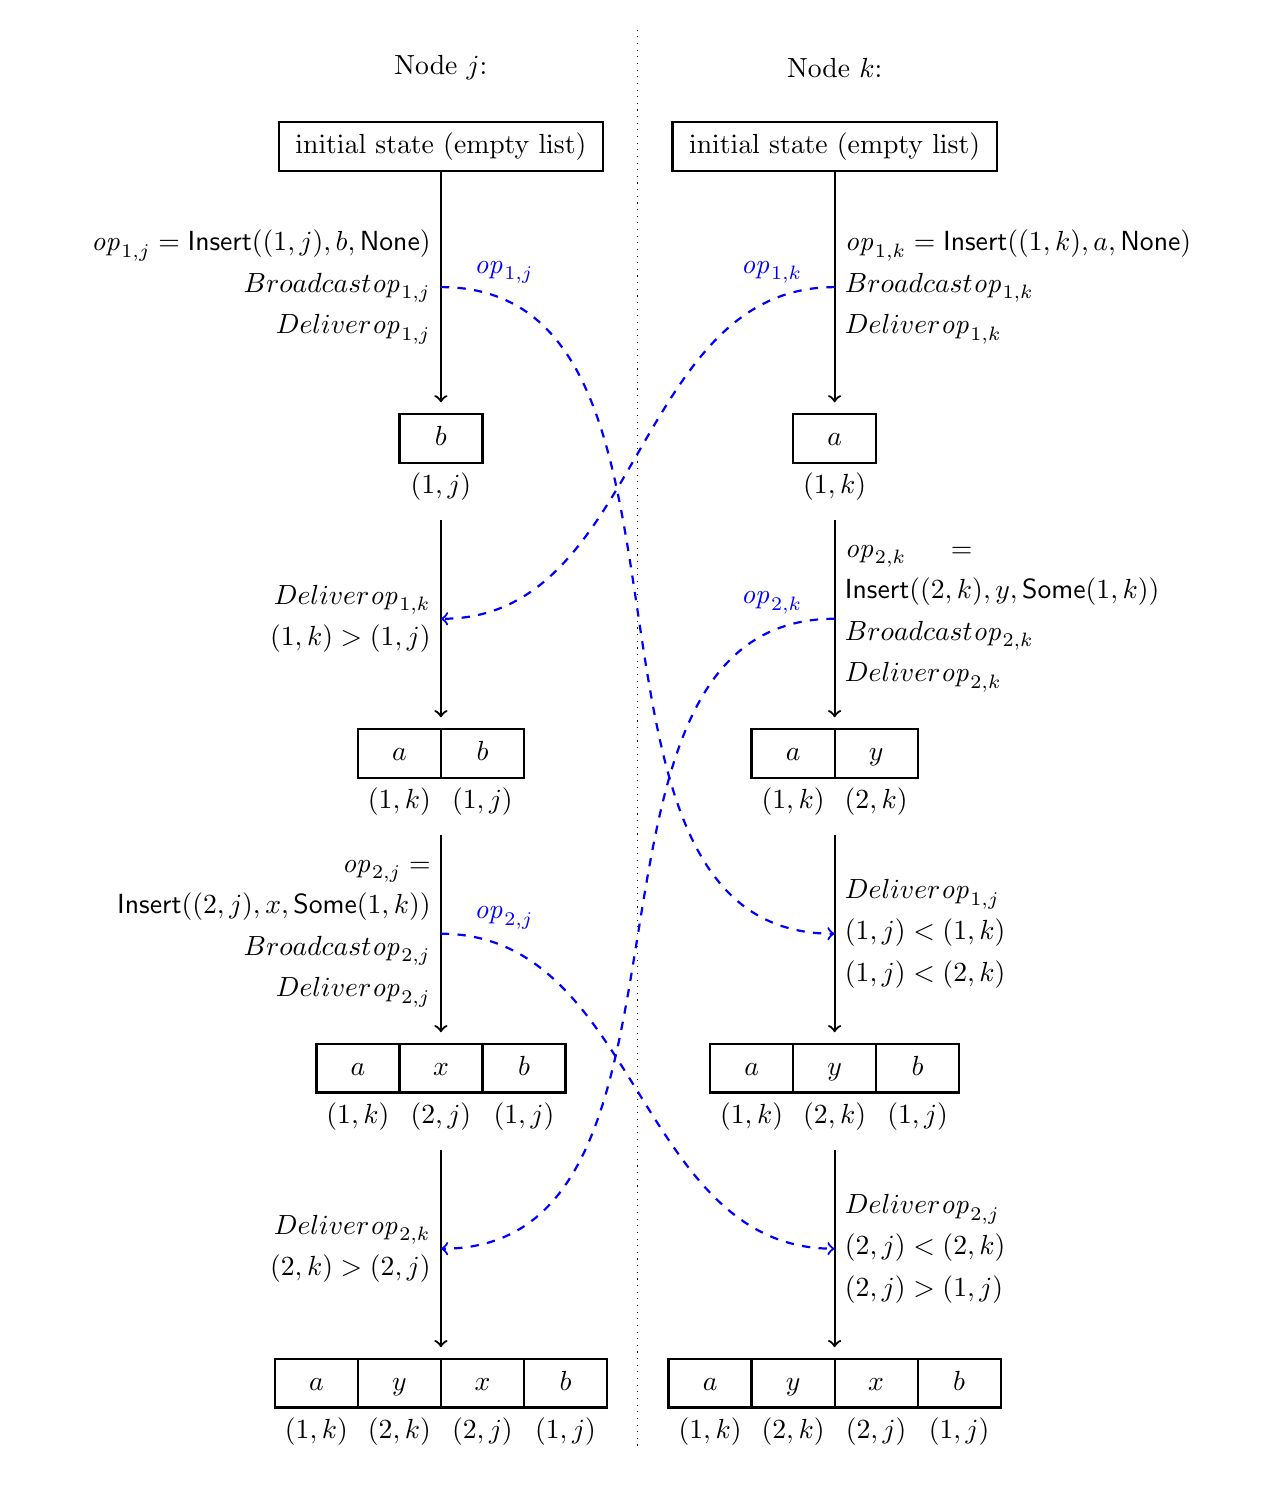
\begin{tikzpicture}[auto,scale=1.0]
\onehalfspacing
\path [draw,dotted] (2.5,-0.5) -- (2.5,17.5);

\tikzstyle{initstate}=[rectangle,draw,inner xsep=6pt,text height=8pt,text depth=3pt]
\tikzstyle{state}=[matrix,column sep={30pt,between origins}]
\tikzstyle{val}=[draw,anchor=base,minimum width=30pt,text height=8pt,text depth=3pt]
\tikzstyle{oid}=[anchor=base]
\tikzstyle{leftevent}=[left,text width=5cm,text ragged left,midway]
\tikzstyle{rightevent}=[right,text width=5cm,text ragged,midway]
\tikzstyle{every path}=[thick,->]

\node (leftR) at (0,17) {Node $j$:};
\node (left1) at (0,16) [initstate] {initial state (empty list)};
\node (left2) at (0,12) [state] {
    \node [val] {$b$};     \\
    \node [oid] {$(1,j)$}; \\
};
\node (left3) at (0,8) [state] {
    \node [val] {$a$};     & \node [val] {$b$};     \\
    \node [oid] {$(1,k)$}; & \node [oid] {$(1,j)$}; \\
};
\node (left4) at (0,4) [state] {
    \node [val] {$a$};     & \node [val] {$x$};     & \node [val] {$b$};     \\
    \node [oid] {$(1,k)$}; & \node [oid] {$(2,j)$}; & \node [oid] {$(1,j)$}; \\
};
\node (left5) at (0,0) [state] {
    \node [val] {$a$};     & \node [val] {$y$};     & \node [val] {$x$};     & \node [val] {$b$};     \\
    \node [oid] {$(1,k)$}; & \node [oid] {$(2,k)$}; & \node [oid] {$(2,j)$}; & \node [oid] {$(1,j)$}; \\
};

\draw (left1) -- (left2) node (send1j) [leftevent] {
    \hfill $\mathit{op}_{1,j} = \mathsf{Insert}((1, j), b, \mathsf{None})$ \\
    \hfill $\text{Broadcast } \mathit{op}_{1,j}$ \\
    \hfill $\text{Deliver } \mathit{op}_{1,j}$ \\
};
\draw (left2) -- (left3) node (recv1k) [leftevent] {
    \hfill $\text{Deliver } \mathit{op}_{1,k}$ \\
    \hfill $(1,k) > (1,j)$ \\
};
\draw (left3) -- (left4) node (send2j) [leftevent] {
    \hfill $\mathit{op}_{2,j} = \mathsf{Insert}((2, j), x, \mathsf{Some}(1,k))$ \\
    \hfill $\text{Broadcast } \mathit{op}_{2,j}$ \\
    \hfill $\text{Deliver } \mathit{op}_{2,j}$ \\
};
\draw (left4) -- (left5) node (recv2k) [leftevent] {
    \hfill $\text{Deliver } \mathit{op}_{2,k}$ \\
    \hfill $(2,k) > (2,j)$ \\
};

\node (rightR) at (5,17) {Node $k$:};
\node (right1) at (5,16) [initstate] {initial state (empty list)};
\node (right2) at (5,12) [state] {
    \node [val] {$a$};     \\
    \node [oid] {$(1,k)$}; \\
};
\node (right3) at (5,8) [state] {
    \node [val] {$a$};     & \node [val] {$y$};     \\
    \node [oid] {$(1,k)$}; & \node [oid] {$(2,k)$}; \\
};
\node (right4) at (5,4) [state] {
    \node [val] {$a$};     & \node [val] {$y$};     & \node [val] {$b$};     \\
    \node [oid] {$(1,k)$}; & \node [oid] {$(2,k)$}; & \node [oid] {$(1,j)$}; \\
};
\node (right5) at (5,0) [state] {
    \node [val] {$a$};     & \node [val] {$y$};     & \node [val] {$x$};     & \node [val] {$b$};     \\
    \node [oid] {$(1,k)$}; & \node [oid] {$(2,k)$}; & \node [oid] {$(2,j)$}; & \node [oid] {$(1,j)$}; \\
};

\draw (right1) -- (right2) node (send1k) [rightevent] {
    $\mathit{op}_{1,k} = \mathsf{Insert}((1, k), a, \mathsf{None})$ \\
    $\text{Broadcast } \mathit{op}_{1,k}$ \\
    $\text{Deliver } \mathit{op}_{1,k}$ \\
};
\draw (right2) -- (right3) node (send2k) [rightevent] {
    $\mathit{op}_{2,k} = \mathsf{Insert}((2, k), y, \mathsf{Some}(1, k))$ \\
    $\text{Broadcast } \mathit{op}_{2,k}$ \\
    $\text{Deliver } \mathit{op}_{2,k}$ \\
};
\draw (right3) -- (right4) node (recv1j) [rightevent] {
    $\text{Deliver } \mathit{op}_{1,j}$ \\
    $(1,j) < (1,k)$ \\
    $(1,j) < (2,k)$ \\
};
\draw (right4) -- (right5) node (recv2j) [rightevent] {
    $\text{Deliver } \mathit{op}_{2,j}$ \\
    $(2,j) < (2,k)$ \\
    $(2,j) > (1,j)$ \\
};

\begin{scope}[dashed,blue]
    \tikzstyle{every node}=[text centered]
    \draw (send1j.east) to [out=0,in=180] (recv1j.west);
    \draw (send2j.east) to [out=0,in=180] (recv2j.west);
    \draw (send1k.west) to [out=180,in=0] (recv1k.east);
    \draw (send2k.west) to [out=180,in=0] (recv2k.east);
    \node at (0.8,14.4) {$\mathit{op}_{1,j}$};
    \node at (0.8, 6.2) {$\mathit{op}_{2,j}$};
    \node at (4.2,14.4) {$\mathit{op}_{1,k}$};
    \node at (4.2,10.2) {$\mathit{op}_{2,k}$};
\end{scope}
\end{tikzpicture}

\caption{RGA example}\label{fig.two-lists}
\end{figure}


\section{High-level proof strategy}
\label{sect.high-level.proof.strategy}

In this section, we provide a high-level overview of our proof strategy, so readers can more easily understand our Isabelle development.

In Section~\ref{sect.abstract.convergence} we present an `abstract convergence theorem' which does not mention networks, nor does it mention any machinery tied to any one particular CRDT implementation. 
Rather, the theorem statement is phrased in terms of purely abstract `events', and functions that lift events into abstract `state formers'.
As a result, the theorem may be viewed purely as a property of preorders, or alternatively as a `distillation' of the notion of SEC convergence, which gives sufficient conditions for convergence in this setting.

In Section~\ref{sect.network} we provide an axiomatic model of causal asynchronous networks, built around a broadcast-deliver event model.
We develop a relation---\emph{happens before}---which captures the notion of `causality' within this network---and is a preorder.
The abstract convergence theorem of Section~\ref{sect.abstract.convergence} therefore applies, and we `compose' this theorem with our network model, to obtain a convergence theorem for our network.

Note that everything mentioned until this point is completely generic---we are not tied to any CRDT implementation.
However, we may now use our abstract convergence theorems to prove concrete convergence theorems for given CRDT implementations.

We present a concrete example in Section~\ref{sect.rga}: a mechanisation of the Replicated Growable Array (RGA).
We first implement the RGA's insert and delete operations, with proofs that each operation commutes with itself, and all operations commute with each other.
Insertion and deletion only commute under various conditions, which are reflected in a constraining of all possible network behaviours to only those that guarantee that the RGA CRDT remains `well behaved'.
This constraining can be viewed as an associated `protocol' for the RGA, detailing valid modes of usage of the data type.
The constrained network provides the right conditions under which all operations commute with each other, and as a corollary of our abstract convergence theorem, we obtain a concrete convergence theorem for our RGA implementation in a constrained network.

%%%%%%%%%%%%%%%%%%%%%%%%%%%%%%%%%%%%%%%%%%%%%%%%%%%%%%%%%%%%%%%%%%%%%%%%%%%%%%%%
% Convergence
%%%%%%%%%%%%%%%%%%%%%%%%%%%%%%%%%%%%%%%%%%%%%%%%%%%%%%%%%%%%%%%%%%%%%%%%%%%%%%%%

\section{Abstract convergence}
\label{sect.abstract.convergence}

In this section we develop an abstract theory of convergence.
The section ends with the presentation of a theorem---imaginatively entitled $\isa{convergence}$---which can be interpreted purely as a result about a certain type of ordering relation.
We will use this theorem, and corollaries of it, in later sections to derive concrete convergence theorems for a CRDT implementation.

Recall that, mathematically, a \emph{preorder} is a reflexive and transitive relation over elements of a carrier set.
In Isabelle/HOL, it is typical to elide carrier sets when working with algebraic or order-theoretic structures, and instead work only with types.
Accordingly, throughout this section, we will work in a setting where an abstract \emph{type} of `events' is fixed with a preorder structure defined over those `events'.
At this point, what `events' are is not specified, only that they exist.
Pre-empting how this preorder relation will eventually be used later in our work, we will refer to the ordering as the \emph{happens before} relation, and will write $\isa{x} \prec \isa{y}$ to indicate that event $\isa{x}$ has \emph{happened before} event $\isa{y}$.
Moreover, we will work in a context where there is a fixed \emph{type} of abstract `states'.
Again, what `states' are need not be specified at this point.
We will also require a means of decoding---or interpreting---an event and obtaining a state transformer, or partial map from states to states.
We therefore assume that there exists a partial function which lifts `events' into state transformers.
We write $\langle\_\rangle$ for this interpretation, or lifting, function.
Concretely, this setting is captured in Isabelle with the following local theory declaration:
\\
\begin{isabellebody}
\ \ \ \ \ \ \ \ \isacommand{locale} happens{\isacharunderscore}before\ {\isacharequal}\ preorder\ hb{\isacharunderscore}weak\ hb\isanewline
\ \ \ \ \ \ \ \ \ \ \isakeyword{for}\ hb{\isacharunderscore}weak\ {\isacharcolon}{\isacharcolon}\ {\isachardoublequoteopen}{\isacharprime}a\ {\isasymRightarrow}\ {\isacharprime}a\ {\isasymRightarrow}\ bool{\isachardoublequoteclose}\ \ {\isacharparenleft}\isakeyword{infix}\ {\isachardoublequoteopen}{\isasympreceq}{\isachardoublequoteclose}\ {\isadigit{5}}{\isadigit{0}}{\isacharparenright}\isanewline
\ \ \ \ \ \ \ \ \ \ \isakeyword{and}\ hb\ {\isacharcolon}{\isacharcolon}\ {\isachardoublequoteopen}{\isacharprime}a\ {\isasymRightarrow}\ {\isacharprime}a\ {\isasymRightarrow}\ bool{\isachardoublequoteclose}\ \ \ \ \ \ \ {\isacharparenleft}\isakeyword{infix}\ {\isachardoublequoteopen}{\isasymprec}{\isachardoublequoteclose}\ {\isadigit{5}}{\isadigit{0}}{\isacharparenright}\ {\isacharplus}\isanewline
\ \ \ \ \ \ \ \ \ \ \isakeyword{fixes}\ interp\ {\isacharcolon}{\isacharcolon}\ {\isachardoublequoteopen}{\isacharprime}a\ {\isasymRightarrow}\ {\isacharprime}b\ {\isasymrightharpoonup}\ {\isacharprime}b{\isachardoublequoteclose}\ {\isacharparenleft}{\isachardoublequoteopen}{\isasymlangle}{\isacharunderscore}{\isasymrangle}{\isachardoublequoteclose}\ {\isacharbrackleft}{\isadigit{0}}{\isacharbrackright}\ {\isadigit{1}}{\isadigit{0}}{\isadigit{0}}{\isadigit{0}}{\isacharparenright}
\end{isabellebody}
\vspace{\baselineskip}
Intuitively, the first three lines of the declaration above create a new local theory called $\isa{happens-before}$ which extends the $\isa{preorder}$ local theory provided by the Isabelle/HOL library.
This $\isa{preorder}$ local theory provides two fixed constants---a weak and a strict ordering---which we rename here to $\isa{hb-weak}$ and $\isa{hb}$.
Throughout, we only use $\isa{hb}$, and ignore $\isa{hb-weak}$.
Further, on the last line of the declaration, we fix a function called $\isa{interp}$, which lifts elements of type ${\isacharprime}a$ into partial functions from ${\isacharprime}b$ to ${\isacharprime}b$.
Here, ${\isacharprime}a$ is our abstract type of `events', whereas ${\isacharprime}b$ is our abstract type of `states'.
Syntax declarations allow us to sugar the $\isa{hb}$ and $\isa{interp}$ constants, as mentioned above.

We say that two events $x$ and $y$ are \emph{concurrent} whenever one does not happens before the other.
That is, $\neg (\isa{x} \prec \isa{y})$ and $\neg (\isa{y} \prec \isa{x})$:
\\
\begin{isabellebody}
\ \ \ \ \ \ \ \ \isacommand{definition} {\isacharparenleft}\isakeyword{in}\ happens{\isacharunderscore}before{\isacharparenright}\ concurrent\ {\isacharcolon}{\isacharcolon}\ {\isachardoublequoteopen}{\isacharprime}a\ {\isasymRightarrow}\ {\isacharprime}a\ {\isasymRightarrow}\ bool{\isachardoublequoteclose}\ {\isacharparenleft}\isakeyword{infix}\ {\isachardoublequoteopen}{\isasymparallel}{\isachardoublequoteclose}\ {\isadigit{5}}{\isadigit{0}}{\isacharparenright}\ \isakeyword{where}\isanewline
\ \ \ \ \ \ \ \ \ \ {\isachardoublequoteopen}x\ {\isasymparallel}\ y\ {\isasymequiv}\ {\isasymnot}\ {\isacharparenleft}x\ {\isasymprec}\ y{\isacharparenright}\ {\isasymand}\ {\isasymnot}\ {\isacharparenleft}y\ {\isasymprec}\ x{\isacharparenright}{\isachardoublequoteclose}
\end{isabellebody}
\vspace{\baselineskip}
Note that this definition is made within the $\isa{happens-before}$ local theory, so has access to the $\isa{hb}$ relation.
We write $x\ {\isasymparallel}\ y$ when two events are concurrent.

We will often work with lists of events that are required to respect the happens before relation.
We say that a list of events \isa{xs} is \emph{hb-consistent}, or simply \emph{consistent}, whenever elements appearing later in the list do not happen before elements appearing earlier in the list.
We capture this idea using an inductive relation in Isabelle:
\\
\begin{isabellebody}
\ \ \ \ \ \ \ \ \isacommand{inductive} hb{\isacharunderscore}consistent\ {\isacharcolon}{\isacharcolon}\ {\isachardoublequoteopen}{\isacharprime}a\ list\ {\isasymRightarrow}\ bool{\isachardoublequoteclose}\ \isakeyword{where}\isanewline
\ \ \ \ \ \ \ \ \ \ {\isachardoublequoteopen}hb{\isacharunderscore}consistent\ {\isacharbrackleft}{\isacharbrackright}{\isachardoublequoteclose}\ {\isacharbar}\isanewline
\ \ \ \ \ \ \ \ \ \ {\isachardoublequoteopen}{\isasymlbrakk}\ hb{\isacharunderscore}consistent\ xs{\isacharsemicolon}\ {\isasymforall}x\ {\isasymin}\ set\ xs{\isachardot}\ {\isasymnot}\ y\ {\isasymprec}\ x\ {\isasymrbrakk}\ {\isasymLongrightarrow}\ hb{\isacharunderscore}consistent\ {\isacharparenleft}xs\ {\isacharat}\ {\isacharbrackleft}y{\isacharbrackright}{\isacharparenright}{\isachardoublequoteclose}
\end{isabellebody}
\vspace{\baselineskip}
Before introducing what it means for two events to be `commutative', we first introduce an auxiliary definition.
For two partial functions, define their \emph{Kleisli arrow composition}, written $f\ {\isasymrhd}\ g$, by:
\\
\begin{isabellebody}
\ \ \ \ \ \ \ \ \isacommand{definition} kleisli\ {\isacharcolon}{\isacharcolon}\ {\isachardoublequoteopen}{\isacharparenleft}{\isacharprime}b\ {\isasymRightarrow}\ {\isacharprime}b\ option{\isacharparenright}\ {\isasymRightarrow}\ {\isacharparenleft}{\isacharprime}b\ {\isasymRightarrow}\ {\isacharprime}b\ option{\isacharparenright}\ {\isasymRightarrow}\ {\isacharparenleft}{\isacharprime}b\ {\isasymRightarrow}\ {\isacharprime}b\ option{\isacharparenright}{\isachardoublequoteclose}\ {\isacharparenleft}\isakeyword{infixr}\ {\isachardoublequoteopen}{\isasymrhd}{\isachardoublequoteclose}\ {\isadigit{6}}{\isadigit{5}}{\isacharparenright}\ \isakeyword{where}\isanewline
\ \ \ \ \ \ \ \ \ \ {\isachardoublequoteopen}f\ {\isasymrhd}\ g\ {\isasymequiv}\ {\isasymlambda}x{\isachardot}\ f\ x\ {\isasymbind}\ {\isacharparenleft}{\isasymlambda}fx{\isachardot}\ g\ fx{\isacharparenright}{\isachardoublequoteclose}
\end{isabellebody}
\vspace{\baselineskip}
Here, $\isasymbind$ is the \emph{monadic bind} operation, defined on the option type that we are using to implement partial functions.
Intuitively, the composition of two partial functions, $f\ {\isasymrhd}\ g$, creates a new partial function that first applies $f$ to its input, then if that succeeds, applies $g$ to the resulting value.
Otherwise, the composition fails.

Using this definition we say that two events, $\isa{x}$ and $\isa{y}$, \emph{commute} whenever $\langle x \rangle {\isasymrhd} \langle y \rangle = \langle y \rangle {\isasymrhd} \langle x \rangle$, i.e. when we can arbitrarily swap the order of the composition of their interpretations.
For our purposes, requiring that this property holds at \emph{every} event is too strong.
Rather, the commutation property is only required to hold at events that are concurrent, as captured in the next definition, which asserts that the interpretation of every pair of concurrent events in a list of events possesses the commutation property:
\\
\begin{isabellebody}
\ \ \ \ \ \ \ \ \isacommand{definition} concurrent{\isacharunderscore}ops{\isacharunderscore}commute\ {\isacharcolon}{\isacharcolon}\ {\isachardoublequoteopen}{\isacharprime}a\ list\ {\isasymRightarrow}\ bool{\isachardoublequoteclose}\ \isakeyword{where}\isanewline
\ \ \ \ \ \ \ \ \ \ {\isachardoublequoteopen}concurrent{\isacharunderscore}ops{\isacharunderscore}commute\ xs\ {\isasymequiv} {\isasymforall}x\ y{\isachardot}\ {\isacharbraceleft}x{\isacharcomma}\ y{\isacharbraceright}\ {\isasymsubseteq}\ set\ xs\ {\isasymlongrightarrow}\ x\ {\isasymparallel}\ y\ {\isasymlongrightarrow}\ {\isasymlangle}x{\isasymrangle}{\isasymrhd}{\isasymlangle}y{\isasymrangle}\ {\isacharequal}\ {\isasymlangle}y{\isasymrangle}{\isasymrhd}{\isasymlangle}x{\isasymrangle}{\isachardoublequoteclose}
\end{isabellebody}
\vspace{\baselineskip}
Suppose $\isa{xs}$ is a list of events.
We define a function, $\isa{apply-operations}$ that `lifts' this list of events into a state transformer.
This is a many-fold analogue of the interpretation function, $\langle-\rangle$, and can be seen as providing an interpretation to the list of events.
Defining this interpretation function is straightforward---we first map $\isa{interp}$ across the list to obtain a list of discrete interpretations of events, and then collectively compose them using the Kleisli arrow composition combinator:
\\
\begin{isabellebody}
\ \ \ \ \ \ \ \ \isacommand{definition} apply{\isacharunderscore}operations\ {\isacharcolon}{\isacharcolon}\ {\isachardoublequoteopen}{\isacharprime}a\ list\ {\isasymRightarrow}\ {\isacharprime}b\ {\isasymrightharpoonup}\ {\isacharprime}b{\isachardoublequoteclose}\ \isakeyword{where}\isanewline
\ \ \ \ \ \ \ \ \ \ {\isachardoublequoteopen}apply{\isacharunderscore}operations\ es\ s\ {\isasymequiv}\ {\isacharparenleft}foldl\ {\isacharparenleft}op\ {\isasymrhd}{\isacharparenright}\ Some\ {\isacharparenleft}map\ interp\ es{\isacharparenright}{\isacharparenright}\ s{\isachardoublequoteclose}
\end{isabellebody}
\vspace{\baselineskip}
We now have sufficient machinery to state our main theorem.
However, before discussing this theorem, we introduce an auxiliary lemma which allows us to manipulate the relative ordering of events within a list of events, without changing the interpretation of that list.
This result will be used in the proof of $\isa{convergence}$, below:
\\
\begin{isabellebody}
\ \ \ \ \ \ \ \ \isacommand{lemma} concurrent{\isacharunderscore}ops{\isacharunderscore}commute{\isacharunderscore}concurrent{\isacharunderscore}set{\isacharcolon}\isanewline
\ \ \ \ \ \ \ \ \ \ \isakeyword{assumes}\ {\isachardoublequoteopen}concurrent{\isacharunderscore}ops{\isacharunderscore}commute\ {\isacharparenleft}prefix{\isacharat}suffix{\isacharat}{\isacharbrackleft}x{\isacharbrackright}{\isacharparenright}{\isachardoublequoteclose}\isanewline
\ \ \ \ \ \ \ \ \ \ \ \ \ \ \isakeyword{and}\ {\isachardoublequoteopen}concurrent{\isacharunderscore}set\ x\ suffix{\isachardoublequoteclose}\isanewline
\ \ \ \ \ \ \ \ \ \ \ \ \ \ \isakeyword{and}\ {\isachardoublequoteopen}distinct\ {\isacharparenleft}prefix\ {\isacharat}\ x\ {\isacharhash}\ suffix{\isacharparenright}{\isachardoublequoteclose}\isanewline
\ \ \ \ \ \ \ \ \ \ \isakeyword{shows}\ {\isachardoublequoteopen}apply{\isacharunderscore}operations\ {\isacharparenleft}prefix\ {\isacharat}\ suffix\ {\isacharat}\ {\isacharbrackleft}x{\isacharbrackright}{\isacharparenright}\ {\isacharequal}\ apply{\isacharunderscore}operations\ {\isacharparenleft}prefix\ {\isacharat}\ x\ {\isacharhash}\ suffix{\isacharparenright}{\isachardoublequoteclose}
\end{isabellebody}
\vspace{\baselineskip}
Here, $\isa{concurrent-set}\ \isa{x}\ \isa{suffix}$ asserts that the event $\isa{x}$ is concurrent with every element of $\isa{suffix}$.
Intuitively, $\isa{concurrent-ops-commute-concurrent-set}$ captures the fact that in a CRDT, it does not matter what the relative ordering a node sees concurrent messages in, as all concurrent messages are guaranteed to commute, and therefore can arbitrarily be reordered.

Using this lemma, and the rest of the machinery defined above, we can now state and then prove our main theorem, which states that two consistent lists of distinct events, which are permutations of each other, in which concurrent operations commute, have the same interpretation:
\\
\begin{isabellebody}
\ \ \ \ \ \ \ \ \isacommand{theorem} convergence{\isacharcolon}\isanewline
\ \ \ \ \ \ \ \ \ \ \isakeyword{assumes}\ {\isachardoublequoteopen}set\ xs\ {\isacharequal}\ set\ ys{\isachardoublequoteclose}\isanewline
\ \ \ \ \ \ \ \ \ \ \ \ \ \ \ \ \isakeyword{and}\ {\isachardoublequoteopen}concurrent{\isacharunderscore}ops{\isacharunderscore}commute\ xs{\isachardoublequoteclose}\ \isakeyword{and}\ {\isachardoublequoteopen}concurrent{\isacharunderscore}ops{\isacharunderscore}commute\ ys{\isachardoublequoteclose}\isanewline
\ \ \ \ \ \ \ \ \ \ \ \ \ \ \ \ \isakeyword{and}\ {\isachardoublequoteopen}distinct\ xs{\isachardoublequoteclose}\ \isakeyword{and}\ {\isachardoublequoteopen}distinct\ ys{\isachardoublequoteclose}\isanewline
\ \ \ \ \ \ \ \ \ \ \ \ \ \ \ \ \isakeyword{and}\ {\isachardoublequoteopen}hb{\isacharunderscore}consistent\ xs{\isachardoublequoteclose}\ \isakeyword{and}\ {\isachardoublequoteopen}hb{\isacharunderscore}consistent\ ys{\isachardoublequoteclose}\isanewline
\ \ \ \ \ \ \ \ \ \ \isakeyword{shows}\ {\isachardoublequoteopen}apply{\isacharunderscore}operations\ xs\ {\isacharequal}\ apply{\isacharunderscore}operations\ ys{\isachardoublequoteclose}\isanewline
\end{isabellebody}

We sketch the proof of this theorem, here.
We proceed by induction on $\isa{xs}$---the case for the empty list is immediate, so we consider the step case only.
Assuming the property holds for \isa{xs}, we prove the case when a new event $\isa{x}$ is added to the end of $\isa{xs}$, that is, $\isa{xs}@[\isa{x}]$.
Since both $\isa{xs}$ and $\isa{ys}$ have the same elements, one may split $\isa{ys}$ such that $\isa{ys = prefix@x@suffix}$ for some suitable lists \isa{prefix} and \isa{suffix}.
Moreover, all events in $\isa{suffix}$ are concurrent with $\isa{x}$.
By the induction hypothesis, $\isa{\isa{apply-operations}\ xs = \isa{apply-operations}\ (prefix@suffix)}$.
We then have a chain of equational reasoning, making use of $\isa{concurrent-ops-commute-concurrent-set}$ to move the element $\isa{x}$ from the back of the list past $\isa{suffix}$, and properties of folds (recalling that $\isa{apply-operations}$ is defined as a fold):
\begin{align*}
  \isa{apply-operations}\ (\isa{xs}@[\isa{x}])
  &= \langle\isa{x}\rangle\ (\isa{apply-operations}\ \isa{xs}) \\
  &= \langle\isa{x}\rangle\ (\isa{apply-operations}\ (\isa{prefix}@\isa{suffix}))\\
  &= \isa{apply-operations} (\isa{prefix}@\isa{suffix}@\isa{x}) \\
  &= \isa{apply-operations} (\isa{prefix}@\isa{x@\isa{suffix}}) \\
  &= \isa{apply-operations}\ ys.
\end{align*}

%%%%%%%%%%%%%%%%%%%%%%%%%%%%%%%%%%%%%%%%%%%%%%%%%%%%%%%%%%%%%%%%%%%%%%%%%%%%%%%%
% Network
%%%%%%%%%%%%%%%%%%%%%%%%%%%%%%%%%%%%%%%%%%%%%%%%%%%%%%%%%%%%%%%%%%%%%%%%%%%%%%%%

\section{Network}
\label{sect.network}

In this section, we incrementally work towards a definition of an asynchronous causal network, considering a number of intermediary abstractions, and important definitions made using those abstractions, along the way.
We conclude the section by demonstrating that our convergence theorem---$\isa{convergence}$, discussed in the previous section---can be `lowered' into an asynchronous causal network, to obtain another convergence theorem.

We first consider a setting characterised by an arbitrary (unbounded) number of `nodes', `replicas', or `processes'.
Precisely what these nodes are, and what their pattern of communication is, if any, is left abstract at this point.
Aside from being unbounded in number, nodes in this setting have two key properties:
\begin{enumerate}
\item
They are uniquely named, and we can always refer to a node with some known unique identifier.
In our setting, we will identify the set of node identifiers with the set of natural numbers.
\item
Each node has an ordered finite history of abstract `events' associated with it---though, at this point we do not specify what these events actually are.
All that can be said is that this history is a `local' history, in that it details a series of network events as the particular node in question perceives them, not a `global' history of all network events seen by some external monitor.
We therefore insist that a node's history is not merely ordered, but has a strict total order structure imposed on it.
Further, every event in a node's history is assumed to be unique.
Uniqueness is a reasonable assumption, as we may use timestamps, globally unique identifiers, or some other disambiguation device attached to concrete messages to ensure that this property holds.
\end{enumerate}
We model the configuration of nodes described above with a local theory in Isabelle, which we call $\isa{node{\isacharunderscore}histories}$:
\\
\begin{isabellebody}
\ \ \ \ \ \ \ \ \isacommand{locale} node{\isacharunderscore}histories\ {\isacharequal}\ \isanewline
\ \ \ \ \ \ \ \ \ \ \isakeyword{fixes}\ history\ {\isacharcolon}{\isacharcolon}\ {\isachardoublequoteopen}nat\ {\isasymRightarrow}\ {\isacharprime}a\ list{\isachardoublequoteclose}\isanewline
\ \ \ \ \ \ \ \ \ \ \isakeyword{assumes}\ histories{\isacharunderscore}distinct{\isacharcolon}\ {\isachardoublequoteopen}distinct\ {\isacharparenleft}history\ i{\isacharparenright}{\isachardoublequoteclose}
\end{isabellebody}
\vspace{\baselineskip}
Here, the history of a node $\isa{i}$ is obtained by using a function fixed by the local theory, $\isa{history}$.
Concretely, we capture the fact that a node's local history is totally ordered by implementing histories as a list of events.
Events are simply modelled as a type variable---here we use $\isa{{\isacharprime}a}$---to ensure that they are completely abstract, with no internal structure.
The $\isa{distinct}$ predicate is an Isabelle/HOL library function which asserts that a list has no repeated elements, upto equality.

Note that the $\isa{node{\isacharunderscore}histories}$ locale is quite general: it can handle both a bounded and unbounded number of nodes.
In the former case, we simply assume that $\isa{history}$ is \emph{finitely supported}, in the sense that all but a bounded number of node histories are `empty', i.e. the function returns the empty list of events at those nodes.

Isabelle lists are finite, and therefore so is a node's history.
As a result, at the end of a node's history, we assume that a node has either \emph{failed} or successfully terminated.
In our model, a node can fail only once, which is modeled by the absence of any further events in the history, and after that it is deemed to have disconnected permanently from the network.
This \emph{crash-stop} abstraction is commonly used by distributed algorithms \cite{Cachin:2011wt}.
Crashes of one node cannot be detected by other nodes: a lack of messages at any given moment might indicate the crash of the sender, message loss, or network delay, and recipients of messages cannot distinguish between these causes.

In the general setting of the $\isa{node{\isacharunderscore}histories}$ local theory, we may define when one event comes before another, at a fixed node.
Writing $\isa{x} \sqsubset^\isa{i} \isa{y}$ for the \emph{comes before} relation at node $\isa{i}$, we assert that this relation holds whenever lists $\isa{xs}$, $\isa{ys}$ and $\isa{zs}$ exist such that $\isa{xs}@[\isa{x}]@\isa{ys}@[\isa{y}]@\isa{zs} = \isa{history\ i}$.
Here $xs@ys$ denotes the appending of list $xs$ to list $ys$.
We define this in Isabelle, like so:
\\
\begin{isabellebody}
\ \ \ \ \ \ \ \ \isacommand{definition} {\isacharparenleft}\isakeyword{in}\ node{\isacharunderscore}histories{\isacharparenright}\ history{\isacharunderscore}order\ {\isacharcolon}{\isacharcolon}\ {\isachardoublequoteopen}{\isacharprime}a\ {\isasymRightarrow}\ nat\ {\isasymRightarrow}\ {\isacharprime}a\ {\isasymRightarrow}\ bool{\isachardoublequoteclose}\ {\isacharparenleft}{\isachardoublequoteopen}{\isacharunderscore}{\isacharslash}\ {\isasymsqsubset}\isactrlsup {\isacharunderscore}{\isacharslash}\ {\isacharunderscore}{\isachardoublequoteclose}\ {\isacharbrackleft}{\isadigit{5}}{\isadigit{0}}{\isacharcomma}{\isadigit{1}}{\isadigit{0}}{\isadigit{0}}{\isadigit{0}}{\isacharcomma}{\isadigit{5}}{\isadigit{0}}{\isacharbrackright}{\isadigit{5}}{\isadigit{0}}{\isacharparenright}\ \isakeyword{where}\isanewline
\ \ \ \ \ \ \ \ \ \ {\isachardoublequoteopen}x\ {\isasymsqsubset}\isactrlsup i\ z\ {\isasymequiv}\ {\isasymexists}xs\ ys\ zs{\isachardot}\ xs{\isacharat}x{\isacharhash}ys{\isacharat}z{\isacharhash}zs\ {\isacharequal}\ history\ i{\isachardoublequoteclose}
\end{isabellebody}
\vspace{\baselineskip}

Often, it will be the case that we are not interested in the entire history of a node, but rather some subcomponent of that history.
In particular, we will often be interested merely in \emph{prefixes} of a node's history, to inspect how the history evolved over time.
We say that a list of events \isa{xs} is a \isa{prefix\ of} the history of node \isa{i} if there exists some list of events \isa{ys} such that their appending forms the history of \isa{i}.
We write $\isa{xs}\ \isa{prefix}\ \isa{of}\ \isa{i}$ when this property holds, and define it formally like so:
\\
\begin{isabellebody}
\ \ \ \ \ \ \ \ \isacommand{definition} {\isacharparenleft}\isakeyword{in}\ node{\isacharunderscore}histories{\isacharparenright}\ prefix{\isacharunderscore}of{\isacharunderscore}node{\isacharunderscore}history\ {\isacharcolon}{\isacharcolon}\ {\isachardoublequoteopen}{\isacharprime}a\ list\ {\isasymRightarrow}\ nat\ {\isasymRightarrow}\ bool{\isachardoublequoteclose}\ {\isacharparenleft}\isakeyword{infix}\ {\isachardoublequoteopen}prefix\ of{\isachardoublequoteclose}\ {\isadigit{5}}{\isadigit{0}}{\isacharparenright}\ \isakeyword{where}\isanewline
\ \ \ \ \ \ \ \ \ \ {\isachardoublequoteopen}xs\ prefix\ of\ i\ {\isasymequiv}\ {\isasymexists}ys{\isachardot}\ xs{\isacharat}ys\ {\isacharequal}\ history\ i{\isachardoublequoteclose}
\end{isabellebody}
\vspace{\baselineskip}
We now move to a slightly less abstract setting.
In particular, the networks that we are modelling consider two different type of events: \emph{broadcast} and \emph{deliver}.
A node can either broadcast a message to every other node on the network, in which case a broadcast event is registered, or can receive a message that has been broadcast by some other node, in which case a deliver event is registered.
In this setting, though broadcast and deliver events have been made concrete, precisely what is being broadcast and delivered is still left unspecified: a message is still an abstract object that will be modelled with a type variable, as by remaining abstract as long as possible, we make our definitions more general.
For operation-based CRDTs messages can be further specified to be a type of operations (like we consider in this work, and where this specification will be made later in this section), or can be specified to be the data structure itself, as in state-based CRDTs.
We define a type of events as a tagged union type, like so:
\\
\begin{isabellebody}
\ \ \ \ \ \ \ \ \isacommand{datatype} {\isacharprime}a\ event\isanewline
\ \ \ \ \ \ \ \ \ \ {\isacharequal}\ Broadcast\ {\isacharprime}a\isanewline
\ \ \ \ \ \ \ \ \ \ {\isacharbar}\ Deliver\ {\isacharprime}a
\end{isabellebody}
\vspace{\baselineskip}
Here, the type variable $\isacharprime\isa{a}$ parameterising the type declaration is used in stead of a concrete representation of messages.

Intuitively, a node can be regarded as a deterministic state machine where each state transition corresponds to a broadcast or deliver event.
We assume that users may query the state of any node at any time, and such queries do not constitute state transitions, since they neither modify the node state nor send or receive any messages.

Our asynchronous networks possess several properties, or `laws', that relate broadcast and deliver messages appearing in the history of various nodes with each other.
In particular, every message received by a node---in a deliver event---must have been broadcast by some node previously.
Using this law, we can assert that no messages are created `out of thin air' by the network itself, and the only source of messages are the nodes of the network.

Our network is not guaranteed to be reliable.
Messages in our network, broadcast by a node, may be delayed, reordered, or even lost entirely, and when a node broadcasts some message, our network does not guarantee that every other node will receive this message in a corresponding deliver event.
The only guarantee that our networks are able to make is that every node will receive its own broadcast messages in delivery events.
When a node recieves its own broadcast messages is not specified, however.
In particular, we make no guarantee that a node will receive its own messages immediately after broadcast, and there may in fact be a significant delay between the two events.

Finally, our network's laws assert that all messages are unique.
If some node has broadcast a message $\isa{m}$, it cannot be the case that some other node has also broadcast that same message.
This is a reasonable assumption to make, as we may always assume that nodes on a real network implementation stamp messages with their own identifiers, when broadcasting, which are already unique by assumption, coupled with a timestamp, or other disambiguating device.

We bundle all of these laws up, defining the notion of a law-abiding asynchronous network, with the $\isa{network}$ local theory, in Isabelle:
\\
\begin{isabellebody}
\ \ \ \ \ \ \ \ \isacommand{locale} network\ {\isacharequal}\ node{\isacharunderscore}histories\ history\ \isakeyword{for}\ history\ {\isacharcolon}{\isacharcolon}\ {\isachardoublequoteopen}nat\ {\isasymRightarrow}\ {\isacharprime}a\ event\ list{\isachardoublequoteclose}\ {\isacharplus}\isanewline
\ \ \ \ \ \ \ \ \ \ \isakeyword{assumes}\ broadcast{\isacharunderscore}before{\isacharunderscore}delivery{\isacharcolon}\ {\isachardoublequoteopen}Deliver\ m\ {\isasymin}\ set\ {\isacharparenleft}history\ i{\isacharparenright}\ {\isasymLongrightarrow}\ {\isasymexists}j{\isachardot}\ Broadcast\ m\ {\isasymsqsubset}\isactrlsup j\ Deliver\ m{\isachardoublequoteclose}\isanewline
\ \ \ \ \ \ \ \ \ \ \ \ \ \ \isakeyword{and}\ deliver{\isacharunderscore}locally{\isacharcolon}\ {\isachardoublequoteopen}Broadcast\ m\ {\isasymin}\ set\ {\isacharparenleft}history\ i{\isacharparenright}\ {\isasymLongrightarrow}\ Broadcast\ m\ {\isasymsqsubset}\isactrlsup i\ Deliver\ m{\isachardoublequoteclose}\isanewline
\ \ \ \ \ \ \ \ \ \ \ \ \ \ \isakeyword{and}\ broadcasts{\isacharunderscore}unique{\isacharcolon}\ {\isachardoublequoteopen}i\ {\isasymnoteq}\ j\ {\isasymLongrightarrow}\ Broadcast\ m\ {\isasymin}\ set\ {\isacharparenleft}history\ i{\isacharparenright}\ {\isasymLongrightarrow}\ Broadcast\ m\ {\isasymnotin}\ set\ {\isacharparenleft}history\ j{\isacharparenright}{\isachardoublequoteclose}
\end{isabellebody}
\vspace{\baselineskip}
Here $\isa{broadcast{\isacharunderscore}before{\isacharunderscore}delivery}$ captures the idea that messages are not created out of thin air, $deliver{\isacharunderscore}locally$ captures the idea that all nodes receive their own broadcast messages, and $broadcasts{\isacharunderscore}unique$ captures the idea that no message can be broadcast by more than one node.

Note also that the first line of the $\isa{network}$ local theory declaration is doing two important things.
First, the $\isa{network}$ local theory is being defined as an \emph{extension} of the $node{\isacharunderscore}histories$ local theory, meaning all functions and axioms fixed or defined within the context of the latter become available in the former.
This is why, for example, the axiom $\isa{broadcast{\isacharunderscore}before{\isacharunderscore}delivery}$---which mentions both the $\isa{history}$ function and the history order relation, defined within the scope of the $node{\isacharunderscore}histories$ local theory---is a well-formed formula.
Second, $\isa{network}$ is not just extending the $node{\isacharunderscore}histories$ local theory, but also \emph{specialising} it at the same time.
The fixed $\isa{history}$ function is now being constrained to return a list of elements of type $\isa{event}$, declared above, rather than some abstract type variable, using the $\isacommand{for}$ construct.

Now that we have some knowledge of broadcast and deliver events, we may define an important concept: the \emph{happens before} relation.
A message (or operation) $\isa{m1}$ is said to \emph{happens before} a message \isa{m2}, whenever:
\begin{enumerate}
\item
If both messages have been broadcast by the same node, and the broadcast event for message $\isa{m1}$ \emph{comes before} the broadcast event for message $\isa{m2}$,
\item
Or, if at some node, the delivery event for message $\isa{m1}$ \emph{comes before} the broadcast event for message $\isa{m2}$,
\item
Or, if there is another event for some message that interpolates the two other events, happening after the event for message $\isa{m1}$, but before the event for message $\isa{m2}$.
\end{enumerate}
We may capture this in Isabelle/HOL using an inductive relation, which we call $\isa{hb}$, alternatively using the syntax $\isa{m1} \prec \isa{m2}$ to assert that $\isa{m1}$ \emph{happens before} $\isa{m2}$ per the definition of $\isa{hb}$:
\\
\begin{isabellebody}
\ \ \ \ \ \ \ \ \isacommand{inductive} {\isacharparenleft}\isakeyword{in}\ network{\isacharparenright}\ hb\ {\isacharcolon}{\isacharcolon}\ {\isachardoublequoteopen}{\isacharprime}a\ {\isasymRightarrow}\ {\isacharprime}a\ {\isasymRightarrow}\ bool{\isachardoublequoteclose}\ \isakeyword{where}\isanewline
\ \ \ \ \ \ \ \ \ \ {\isachardoublequoteopen}{\isasymlbrakk}\ Broadcast\ m{\isadigit{1}}\ {\isasymsqsubset}\isactrlsup i\ Broadcast\ m{\isadigit{2}}\ {\isasymrbrakk}\ {\isasymLongrightarrow}\ m{\isadigit{1}}\ $\prec$\ m{\isadigit{2}}{\isachardoublequoteclose}\ {\isacharbar}\isanewline
\ \ \ \ \ \ \ \ \ \ {\isachardoublequoteopen}{\isasymlbrakk}\ Deliver\ m{\isadigit{1}}\ {\isasymsqsubset}\isactrlsup i\ Broadcast\ m{\isadigit{2}}\ {\isasymrbrakk}\ {\isasymLongrightarrow}\ m{\isadigit{1}}\ $\prec$\ m{\isadigit{2}}{\isachardoublequoteclose}\ {\isacharbar}\isanewline
\ \ \ \ \ \ \ \ \ \ {\isachardoublequoteopen}{\isasymlbrakk}\ m{\isadigit{1}}\ $\prec$\  m{\isadigit{2}}{\isacharsemicolon}\ m{\isadigit{2}}\ $\prec$\ m{\isadigit{3}}\ {\isasymrbrakk}\ {\isasymLongrightarrow}\ m{\isadigit{1}}\ $\prec$\ m{\isadigit{3}}{\isachardoublequoteclose}
\end{isabellebody}
\vspace{\baselineskip}
Each of the three clauses in the definition of $\isa{hb}$ above corresponds to one of the three conditions previously enumerated.
The fact that the \emph{happens before} relation is a preorder is easily established, and is omitted here.

Our convergence proof requires that our asynchronous networks abide by an additional law: \emph{causality}.
We say that an asynchronous network is \emph{causal} if delivery of events corresponding to messages $\isa{m1}$ and $\isa{m2}$ at a node respect the happens before relationship between those two events.
In particular, we only require that the happens before relation's ordering is respected at nodes which have the delivery of the second message in their local histories.

Since causal asynchronous networks are a special form of asynchronous network, we describe these networks with a new local theory.
This increases modularity and makes our definitions adaptable for other formalisations that do not depend on causality:
\\
\begin{isabellebody}
\ \ \ \ \ \ \ \ \isacommand{locale} causal{\isacharunderscore}network\ {\isacharequal}\ network\ {\isacharplus}\isanewline
\ \ \ \ \ \ \ \ \ \ \ \isakeyword{assumes}\ causal{\isacharunderscore}delivery{\isacharcolon}\ {\isachardoublequoteopen}Deliver\ m{\isadigit{2}}\ {\isasymin}\ set\ {\isacharparenleft}history\ j{\isacharparenright}\ {\isasymLongrightarrow}\ m{\isadigit{1}}\ $\prec$\ m{\isadigit{2}}\ {\isasymLongrightarrow}\ Deliver\ m{\isadigit{1}}\ {\isasymsqsubset}\isactrlsup j\ Deliver\ m{\isadigit{2}}{\isachardoublequoteclose}
\end{isabellebody}
\vspace{\baselineskip}
Here, $causal{\isacharunderscore}delivery$ captures the causality constraint, described above, that asynchronous causal networks must satisfy.
Note also that the local theory $causal{\isacharunderscore}network$ is declared to be an extension of the $network$ local theory on the first line of the declaration above.

At this point, we now have sufficient machinery to instantiate the \isa{happens-before} local theory that was defined in Section~\ref{sect.abstract.convergence}.
Doing this requires that we provide a concrete implementation for the happens before relation fixed by that local theory and thereafter proving that it forms indeed a preorder, so this proof obligation can easily be discharged.
Here, we will use the $\isa{hb}$ relation, defined earlier in this section, as that implementation, and we have already noted that this relation does indeed satisfies the laws of a preorder.
Once interpreted, all functions, definitions, and theorems made within the \isa{happens-before} locale become available to use in the locale \isa{network}, prefixed by \isa{hb}--- a `composing' of the definitions made within the $\isa{happens-before}$ local theory with our $\isa{hb}$ inductive relation.
In particular, the definitions of \isa{hb.concurrent}, \isa{hb.concurrent-ops-commute} and \isa{hb.hb-consistent}; and the convergence theorem \isa{hb.convergence}.
This instantiation is achieved in Isabelle using a \isa{sublocale} statement:
\\
\begin{isabellebody}
\ \ \ \ \ \ \ \ \isacommand{sublocale} hb{\isacharcolon}\ happens{\isacharunderscore}before\ weak{\isacharunderscore}hb\ hb
\end{isabellebody}
\vspace{\baselineskip}
\noindent
We end this section by describing an analogue of the convergence theorem in Section~\ref{sect.abstract.convergence}.

We first define a function, $node{\isacharunderscore}deliver{\isacharunderscore}messages$ which filters a list of events to obtain a list of delivered messages.
Note in particular that deliver events for messages are the only type of network event that can and will modify the state of a CRDT.
We therefore only need to consider these messages in our convergence theorem.
We elide the definition of $node{\isacharunderscore}deliver{\isacharunderscore}messages$ here, as it is a simple filter/map of a node's local history.

A node's local history satisfies two important properties in causal asynchronous networks.
First, the delivered messages of a prefix of a node's history are necessarily distinct:
\\
\begin{isabellebody}
\ \ \ \ \ \ \ \ \isacommand{lemma} {\isacharparenleft}\isakeyword{in}\ causal{\isacharunderscore}network{\isacharparenright}\ node{\isacharunderscore}deliver{\isacharunderscore}messages{\isacharunderscore}distinct{\isacharcolon}\isanewline
\ \ \ \ \ \ \ \ \ \ \isakeyword{assumes}\ {\isachardoublequoteopen}xs\ prefix\ of\ i{\isachardoublequoteclose}\isanewline
\ \ \ \ \ \ \ \ \ \ \isakeyword{shows}\ {\isachardoublequoteopen}distinct\ {\isacharparenleft}node{\isacharunderscore}deliver{\isacharunderscore}messages\ xs{\isacharparenright}{\isachardoublequoteclose}
\end{isabellebody}
\vspace{\baselineskip}
Second, the delivered messages of a prefix of a node's history are also necessarily compatible with the happens before relation, the $hb$ relation defined above:
\\
\begin{isabellebody}
\ \ \ \ \ \ \ \ \isacommand{lemma} {\isacharparenleft}\isakeyword{in}\ causal{\isacharunderscore}network{\isacharparenright}\ hb{\isacharunderscore}consistent{\isacharunderscore}prefix{\isacharcolon}\isanewline
\ \ \ \ \ \ \ \ \ \ \isakeyword{assumes}\ {\isachardoublequoteopen}xs\ prefix\ of\ i{\isachardoublequoteclose}\isanewline
\ \ \ \ \ \ \ \ \ \ \isakeyword{shows}\ {\isachardoublequoteopen}hb{\isachardot}hb{\isacharunderscore}consistent\ {\isacharparenleft}node{\isacharunderscore}deliver{\isacharunderscore}messages\ xs{\isacharparenright}{\isachardoublequoteclose}
\end{isabellebody}
\vspace{\baselineskip}
Taken together, these two properties imply that at any point in time, the messages received by a node are distinct and satisfy the consistency requirement defined in Section~\ref{sect.abstract.convergence}.
With this, the abstract convergence theorem of Section~\ref{sect.abstract.convergence} can be refined to consider the prefixes of two different nodes with the same set of delivered messages.
We then obtain a theorem that states that if concurrent messages commute, then both nodes converge to the same state:
\\
\begin{isabellebody}
\ \ \ \ \ \ \ \ \isacommand{corollary} {\isacharparenleft}\isakeyword{in}\ causal{\isacharunderscore}network{\isacharparenright}\ network{\isacharunderscore}convergence{\isacharcolon}\isanewline
\ \ \ \ \ \ \ \ \ \ \isakeyword{assumes}\ {\isachardoublequoteopen}xs\ prefix\ of\ i{\isachardoublequoteclose} \isakeyword{and}\ {\isachardoublequoteopen}ys\ prefix\ of\ j{\isachardoublequoteclose}\isanewline
\ \ \ \ \ \ \ \ \ \ \ \ \ \ \isakeyword{and}\ {\isachardoublequoteopen}set\ {\isacharparenleft}node{\isacharunderscore}deliver{\isacharunderscore}messages\ xs{\isacharparenright}\ {\isacharequal}\ set\ {\isacharparenleft}node{\isacharunderscore}deliver{\isacharunderscore}messages\ ys{\isacharparenright}{\isachardoublequoteclose}\isanewline
\ \ \ \ \ \ \ \ \ \ \ \ \ \ \isakeyword{and}\ {\isachardoublequoteopen}concurrent{\isacharunderscore}ops{\isacharunderscore}commute\ {\isacharparenleft}node{\isacharunderscore}deliver{\isacharunderscore}messages\ xs{\isacharparenright}{\isachardoublequoteclose} \isakeyword{and}\ {\isachardoublequoteopen}concurrent{\isacharunderscore}ops{\isacharunderscore}commute\ {\isacharparenleft}node{\isacharunderscore}deliver{\isacharunderscore}messages\ ys{\isacharparenright}{\isachardoublequoteclose}\isanewline
\ \ \ \ \ \ \ \ \ \ \isakeyword{shows}\ {\isachardoublequoteopen}hb.apply{\isacharunderscore}operations\ {\isacharparenleft}node{\isacharunderscore}deliver{\isacharunderscore}messages\ xs{\isacharparenright}\ {\isacharequal}\ hb.apply{\isacharunderscore}operations\ {\isacharparenleft}node{\isacharunderscore}deliver{\isacharunderscore}messages\ ys{\isacharparenright}{\isachardoublequoteclose}
\end{isabellebody}

%%%%%%%%%%%%%%%%%%%%%%%%%%%%%%%%%%%%%%%%%%%%%%%%%%%%%%%%%%%%%%%%%%%%%%%%%%%%%%%%
% RGA
%%%%%%%%%%%%%%%%%%%%%%%%%%%%%%%%%%%%%%%%%%%%%%%%%%%%%%%%%%%%%%%%%%%%%%%%%%%%%%%%

\section{Replicated Growable Array}
\label{sect.rga}

In this section, we discuss our implementation of the Replicated Growable Array (RGA) CRDT, and various theorems related to its correctness.
We finish the section with a proof that the RGA implementation converges.

\noindent
\paragraph{Definition}
The RGA is a replicated sequential data type supporting two operations: \emph{insert} and \emph{delete}.
Three aspects of the RGA ensure convergence.
First, all elements stored in the list have associated identifiers, which are totally ordered, with the insertion operation using this ordering to find a suitable index to place an element into the list.
Second, the RGA's delete operation does not \emph{remove} elements from the list, but merely flips a `tombstone' flag associated with the element to indicate that the element is marked as having been deleted.
Properly working with the RGA---for example in an application which wishes to print out the elements stored in the array---therefore requires that the application layer be made aware of these tombstones.
Finally, the RGA---like many CRDTs---comes with preconditions on its operations that are guaranteed by a `protocol', or restriction on message event histories within the network.
These restrictions are reflected as hypotheses in our convergence theorems, presented below, and are reified as a new local theory, within Isabelle, specialising the network local theories presented in previous sections to capture those network behaviours that respect the RGA protocol.
This will be further discussed below.

Accordingly, we fix a type of `elements' which will be stored in our RGA implementation:
\\
\begin{isabellebody}
\ \ \ \ \ \ \ \ \isacommand{type{\isacharunderscore}synonym} {\isacharparenleft}{\isacharprime}id{\isacharcomma}\ {\isacharprime}v{\isacharparenright}\ elt\ {\isacharequal}\ {\isachardoublequoteopen}{\isacharprime}id\ {\isasymtimes}\ {\isacharprime}v\ {\isasymtimes}\ bool{\isachardoublequoteclose}%
\end{isabellebody}
\vspace{\baselineskip}
Here, we instruct Isabelle/HOL to treat the type ${\isacharparenleft}{\isacharprime}id{\isacharcomma}\ {\isacharprime}v{\isacharparenright}\ elt$ as an alias for the product type ${\isacharprime}id\ {\isasymtimes}\ {\isacharprime}v\ {\isasymtimes}\ bool$.
Note that the type alias is parameterised by two type variables, ${\isacharprime}id$ and ${\isacharprime}v$, the former of which stands for some arbitrary type of identifiers\footnote{Almost always, we will be working in a context where the type variable ${\isacharprime}id$ is assumed to have an associated total (or linear) order.
We will indicate this syntactically to Isabelle using the syntax ${\isacharprime}id{\isacharcolon}{\isacharcolon}{\isacharbraceleft}\isa{linorder}{\isacharbraceright}$ in type expressions, which asserts that ${\isacharprime}id$ should be substitutable only for types with an associated total order.
Here, $\isa{linorder}$ is the name of a type class supplied by the Isabelle/HOL library, capturing the notion of a total ordering.}, whilst the latter stands for the type of data we will be storing in the RGA.
The last component of the product is the boolean tombstone flag, indicating deletion, as discussed above.
By convention, we assume this flag having the value $\isa{True}$ indicates that the containing element has been deleted.

We now define the RGA's insertion operation.
The RGA's insertion operates in two modes, reflecting the data type's use as a means of implementing collaborative editing applications.
In one mode, an element may be inserted automatically into the body of the array, using the ordered identifiers of each element as a guide for where to place the new element.
In another mode, the user may specifically request that an element is placed \emph{after} another.
As a result in our mechanisation we found it convenient for later proofs to factor the definition of insertion into two functions.
The first function, $\isa{insert-body}$ never fails, and is used by the second (and main) insertion function, $\isa{insert}$, to insert an element within the body of the list.

The function $\isa{insert\ xs\ e\ i}$ performs a case analysis on its third argument, $\isa{i}$.
If $\isa{i}$ is $\isa{None}$, then this is taken to mean that the user wishes the element to be placed in the body of the ordered list, and $\isa{insert-body}$ is therefore immediately called.
Otherwise, $\isa{i}$ is of the form $\isa{Some\ i'}$ for some identifier $\isa{i'}$, in which case the user wishes the new element to appear after some existing element in the list.
This is done recursively by $\isa{insert}$ itself.
Note that \isa{insert} is a partial function, if an element with identifier \isa{i} is not found in the list \isa{xs}, the function returns \isa{None}, indicating failure.

The definition of the $\isa{insert-body}$ function is straightforward, with the function being defined by recursion over the list of elements, using Isabelle's pattern matching to destructure the list:
\\
\begin{isabellebody}
\ \ \ \ \ \ \ \ \isacommand{fun} insert{\isacharunderscore}body\ {\isacharcolon}{\isacharcolon}\ {\isachardoublequoteopen}{\isacharparenleft}{\isacharprime}id{\isacharcolon}{\isacharcolon}{\isacharbraceleft}linorder{\isacharbraceright}{\isacharcomma}\ {\isacharprime}v{\isacharparenright}\ elt\ list\ {\isasymRightarrow}\ {\isacharparenleft}{\isacharprime}id{\isacharcomma}\ {\isacharprime}v{\isacharparenright}\ elt\ {\isasymRightarrow}\ {\isacharparenleft}{\isacharprime}id{\isacharcomma}\ {\isacharprime}v{\isacharparenright}\ elt\ list{\isachardoublequoteclose}\ \isakeyword{where}\isanewline
\ \ \ \ \ \ \ \ \ \ {\isachardoublequoteopen}insert{\isacharunderscore}body\ {\isacharbrackleft}{\isacharbrackright}\ \ \ \ \ e\ {\isacharequal}\ {\isacharbrackleft}e{\isacharbrackright}{\isachardoublequoteclose}\ {\isacharbar}\isanewline
\ \ \ \ \ \ \ \ \ \ {\isachardoublequoteopen}insert{\isacharunderscore}body\ {\isacharparenleft}x{\isacharhash}xs{\isacharparenright}\ e\ {\isacharequal}\isanewline
\ \ \ \ \ \ \ \ \ \ \ \ \ {\isacharparenleft}if\ fst\ x\ {\isacharless}\ fst\ e\ then\isanewline
\ \ \ \ \ \ \ \ \ \ \ \ \ \ \ \ e{\isacharhash}x{\isacharhash}xs\isanewline
\ \ \ \ \ \ \ \ \ \ \ \ \ \ else\ x{\isacharhash}insert{\isacharunderscore}body\ xs\ e{\isacharparenright}{\isachardoublequoteclose}
\end{isabellebody}
\vspace{\baselineskip}
Note here that $\isa{fst}$ is an Isabelle library function that returns the first component of a tuple.
Recalling the definition of the $\isa{elt}$ type alias, we see that $\isa{fst}\ x < \isa{fst}\ e$ in the conditional above is comparing the identifiers of the two elements.
The definition of $\isa{insert}$ is slightly more complicated, but also essentially follows a recursive scheme, pattern matching on both the input list, and the third argument---i.e. the position where to place the new element in the list:
\\
\begin{isabellebody}
\ \ \ \ \ \ \ \ \isacommand{fun} insert\ {\isacharcolon}{\isacharcolon}\ {\isachardoublequoteopen}{\isacharparenleft}{\isacharprime}id{\isacharcolon}{\isacharcolon}{\isacharbraceleft}linorder{\isacharbraceright}{\isacharcomma}\ {\isacharprime}v{\isacharparenright}\ elt\ list\ {\isasymRightarrow}\ {\isacharparenleft}{\isacharprime}id{\isacharcomma}\ {\isacharprime}v{\isacharparenright}\ elt\ {\isasymRightarrow}\ {\isacharprime}id\ option\ {\isasymrightharpoonup}\ {\isacharparenleft}{\isacharprime}id{\isacharcomma}\ {\isacharprime}v{\isacharparenright}\ elt\ list{\isachardoublequoteclose}\ \isakeyword{where}\isanewline
\ \ \ \ \ \ \ \ \ \ {\isachardoublequoteopen}insert\ xs\ \ \ \ \ e\ None\ \ \ \ \ {\isacharequal}\ Some\ {\isacharparenleft}insert{\isacharunderscore}body\ xs\ e{\isacharparenright}{\isachardoublequoteclose}\ {\isacharbar}\isanewline
\ \ \ \ \ \ \ \ \ \ {\isachardoublequoteopen}insert\ {\isacharbrackleft}{\isacharbrackright}\ \ \ \ \ e\ {\isacharparenleft}Some\ i{\isacharparenright}\ {\isacharequal}\ None{\isachardoublequoteclose}\ {\isacharbar}\isanewline
\ \ \ \ \ \ \ \ \ \ {\isachardoublequoteopen}insert\ {\isacharparenleft}x{\isacharhash}xs{\isacharparenright}\ e\ {\isacharparenleft}Some\ i{\isacharparenright}\ {\isacharequal}\isanewline
\ \ \ \ \ \ \ \ \ \ \ \ \ {\isacharparenleft}if\ fst\ x\ {\isacharequal}\ i\ then\isanewline
\ \ \ \ \ \ \ \ \ \ \ \ \ \ \ \ Some\ {\isacharparenleft}x{\isacharhash}insert{\isacharunderscore}body\ xs\ e{\isacharparenright}\isanewline
\ \ \ \ \ \ \ \ \ \ \ \ \ \ else\isanewline
\ \ \ \ \ \ \ \ \ \ \ \ \ \ \ \ do\ {\isacharbraceleft}\ t\ {\isasymleftarrow}\ insert\ xs\ e\ {\isacharparenleft}Some\ i{\isacharparenright}\isanewline
\ \ \ \ \ \ \ \ \ \ \ \ \ \ \ \ \ \ \ {\isacharsemicolon}\ Some\ {\isacharparenleft}x{\isacharhash}t{\isacharparenright}\isanewline
\ \ \ \ \ \ \ \ \ \ \ \ \ \ \ \ \ \ \ {\isacharbraceright}{\isacharparenright}{\isachardoublequoteclose}
\end{isabellebody}
\vspace{\baselineskip}
Here, $do {\isacharbraceleft} \ldots {\isacharbraceright}$ is a \emph{monadic sequencing block}, containing code in the option monad that could possibly fail.
This block will collapse with a failure (i.e. $\isa{None}$) return value if any intermediate computation in the block fails.

Compared to insertion, the delete operation for the RGA is more straightforward---it simply searches recursively for the element with a given identifier and change its flag to $\isa{True}$.
As previously mentioned, by convention we take this to mean that the element has been deleted:
\\
\begin{isabellebody}
\ \ \ \ \ \ \ \ \isacommand{fun} delete\ {\isacharcolon}{\isacharcolon}\ {\isachardoublequoteopen}{\isacharparenleft}{\isacharprime}id{\isacharcolon}{\isacharcolon}{\isacharbraceleft}linorder{\isacharbraceright}{\isacharcomma}\ {\isacharprime}v{\isacharparenright}\ elt\ list\ {\isasymRightarrow}\ {\isacharprime}id\ {\isasymrightharpoonup}\ {\isacharparenleft}{\isacharprime}id{\isacharcomma}\ {\isacharprime}v{\isacharparenright}\ elt\ list{\isachardoublequoteclose}\ \isakeyword{where}\isanewline
\ \ \ \ \ \ \ \ \ \ {\isachardoublequoteopen}delete\ {\isacharbrackleft}{\isacharbrackright}\ \ \ \ \ \ \ \ \ \ \ \ \ \ \ \ \ i\ {\isacharequal}\ None{\isachardoublequoteclose}\ {\isacharbar}\isanewline
\ \ \ \ \ \ \ \ \ \ {\isachardoublequoteopen}delete\ {\isacharparenleft}{\isacharparenleft}i{\isacharprime}{\isacharcomma}\ v{\isacharcomma}\ flag{\isacharparenright}{\isacharhash}xs{\isacharparenright}\ i\ {\isacharequal}\ \isanewline
\ \ \ \ \ \ \ \ \ \ \ \ \ {\isacharparenleft}if\ i{\isacharprime}\ {\isacharequal}\ i\ then\isanewline
\ \ \ \ \ \ \ \ \ \ \ \ \ \ \ \ Some\ {\isacharparenleft}{\isacharparenleft}i{\isacharprime}{\isacharcomma}\ v{\isacharcomma}\ True{\isacharparenright}{\isacharhash}xs{\isacharparenright}\isanewline
\ \ \ \ \ \ \ \ \ \ \ \ \ \ else\isanewline
\ \ \ \ \ \ \ \ \ \ \ \ \ \ \ \ do\ {\isacharbraceleft}\ t\ {\isasymleftarrow}\ delete\ xs\ i\isanewline
\ \ \ \ \ \ \ \ \ \ \ \ \ \ \ \ \ \ \ {\isacharsemicolon}\ Some\ {\isacharparenleft}{\isacharparenleft}i{\isacharprime}{\isacharcomma}v{\isacharcomma}flag{\isacharparenright}{\isacharhash}t{\isacharparenright}\isanewline
\ \ \ \ \ \ \ \ \ \ \ \ \ \ \ \ \ \ \ {\isacharbraceright}{\isacharparenright}{\isachardoublequoteclose}%
\end{isabellebody}
\vspace{\baselineskip}
Note that the operations presented here are deliberately inefficient, in order to make them easier to reason with.
One can see our implementations of $\isa{insert-body}$, $\isa{insert}$, and $\isa{delete}$ as functional specifications for RGAs, which could be refined into more efficient algorithms using data refinement, if desired.

We mention here, briefly, two useful lemmas that will be used later, and which characterise the conditions under which the $\isa{insert}$ and the $\isa{delete}$ functions can fail, i.e. return $\isa{None}$.

For $\isa{insert\ xs\ e\ i}$, the function will will never fail if $\isa{i}$ is $\isa{None}$ or there exists an element in $\isa{xs}$ with identifier $\isa{i}$.
This is captured by the lemma $insert{\isacharunderscore}no{\isacharunderscore}failure$:
\\
\begin{isabellebody}
\ \ \ \ \ \ \ \ \isacommand{lemma} insert{\isacharunderscore}no{\isacharunderscore}failure{\isacharcolon}\isanewline
\ \ \ \ \ \ \ \ \ \ \isakeyword{assumes}\ {\isachardoublequoteopen}i\ {\isacharequal}\ None\ {\isasymor}\ {\isacharparenleft}{\isasymexists}i{\isacharprime}{\isachardot}\ i\ {\isacharequal}\ Some\ i{\isacharprime}\ {\isasymand}\ i{\isacharprime}\ {\isasymin}\ fst\ {\isacharbackquote}\ set\ xs{\isacharparenright}{\isachardoublequoteclose}\isanewline
\ \ \ \ \ \ \ \ \ \ \isakeyword{shows}\ \ \ {\isachardoublequoteopen}{\isasymexists}xs{\isacharprime}{\isachardot}\ insert\ xs\ e\ i\ {\isacharequal}\ Some\ xs{\isacharprime}{\isachardoublequoteclose}
\end{isabellebody}
\vspace{\baselineskip}
Similarly, for $\isa{delete\ xs\ i}$, the function will never fail if there exists an element in $\isa{xs}$ with identifier $\isa{i}$.
This is captured by the lemma $\isa{delete{\isacharunderscore}no{\isacharunderscore}failure}$:
\\
\begin{isabellebody}
\ \ \ \ \ \ \ \ \isacommand{lemma} delete{\isacharunderscore}no{\isacharunderscore}failure{\isacharcolon}\isanewline
\ \ \ \ \ \ \ \ \ \ \isakeyword{assumes}\ {\isachardoublequoteopen}i\ {\isasymin}\ fst\ {\isacharbackquote}\ set\ xs{\isachardoublequoteclose}\isanewline
\ \ \ \ \ \ \ \ \ \ \isakeyword{shows}\ \ \ {\isachardoublequoteopen}{\isasymexists}xs{\isacharprime}{\isachardot}\ delete\ xs\ i\ {\isacharequal}\ Some\ xs{\isacharprime}{\isachardoublequoteclose}\isanewline
\end{isabellebody}

\paragraph{Commutativity}

We now prove that $\isa{insert}$ and $\isa{delete}$ commute.
Technical lemmas relating to the commutation of $\isa{insert-body}$ will be elided.
We call two insertion operations---$\isa{insert\ xs\ e1\ i1}$ and $\isa{insert\ xs\ e2\ i2}$---`concurrent' whenever $\isa{i1}$ is not the identifier of $\isa{e2}$, and vice versa.
Assuming that every element already present in the list $\isa{xs}$ has a unique identifier---and therefore the identifiers of $\isa{e1}$ and $\isa{e2}$ are distinct---we can show that $\isa{insert}$ commutes with itself on concurrent insertion operations, in the following lemma:
\\
\begin{isabellebody}
\ \ \ \ \ \ \ \ \isacommand{lemma} insert{\isacharunderscore}commutes{\isacharcolon}\isanewline
\ \ \ \ \ \ \ \ \ \ \isakeyword{assumes}\ {\isachardoublequoteopen}fst\ e{\isadigit{1}}\ {\isasymnoteq}\ fst\ e{\isadigit{2}}{\isachardoublequoteclose}\isanewline
\ \ \ \ \ \ \ \ \ \ \ \ \isakeyword{and}\ {\isachardoublequoteopen}i{\isadigit{1}}\ {\isacharequal}\ None\ {\isasymor}\ i{\isadigit{1}}\ {\isasymnoteq}\ Some\ {\isacharparenleft}fst\ e{\isadigit{2}}{\isacharparenright}{\isachardoublequoteclose}\isanewline
\ \ \ \ \ \ \ \ \ \ \ \ \isakeyword{and}\ {\isachardoublequoteopen}i{\isadigit{2}}\ {\isacharequal}\ None\ {\isasymor}\ i{\isadigit{2}}\ {\isasymnoteq}\ Some\ {\isacharparenleft}fst\ e{\isadigit{1}}{\isacharparenright}{\isachardoublequoteclose}\isanewline
\ \ \ \ \ \ \ \ \ \ \isakeyword{shows}\ \ \ {\isachardoublequoteopen}do\ {\isacharbraceleft}\ ys\ {\isasymleftarrow}\ insert\ xs\ e{\isadigit{1}}\ i{\isadigit{1}}{\isacharsemicolon}\ insert\ ys\ e{\isadigit{2}}\ i{\isadigit{2}}\ {\isacharbraceright}\ {\isacharequal}\ do\ {\isacharbraceleft}\ ys\ {\isasymleftarrow}\ insert\ xs\ e{\isadigit{2}}\ i{\isadigit{2}}{\isacharsemicolon}\ insert\ ys\ e{\isadigit{1}}\ i{\isadigit{1}}\ {\isacharbraceright}{\isachardoublequoteclose}
\end{isabellebody}
\vspace{\baselineskip}
It is straightforward to demonstrate that $\isa{delete}$ will always commute with itself, on concurrent and non-concurrent operations alike, as in the following lemma:
\\
\begin{isabellebody}
\ \ \ \ \ \ \ \ \isacommand{lemma} delete{\isacharunderscore}commutes{\isacharcolon}\isanewline
\ \ \ \ \ \ \ \ \ \ \isakeyword{shows}\ {\isachardoublequoteopen}do\ {\isacharbraceleft}\ ys\ {\isasymleftarrow}\ delete\ xs\ i{\isadigit{1}}{\isacharsemicolon}\ delete\ ys\ i{\isadigit{2}}\ {\isacharbraceright}\ {\isacharequal}\ do\ {\isacharbraceleft}\ ys\ {\isasymleftarrow}\ delete\ xs\ i{\isadigit{2}}{\isacharsemicolon}\ delete\ ys\ i{\isadigit{1}}\ {\isacharbraceright}{\isachardoublequoteclose}
\end{isabellebody}
\vspace{\baselineskip}
Finally, $\isa{delete}$ commutes with insertion operations whenever the element to be deleted is not the same as the element to be inserted---in other words, when the two operations are concurrent.
This is shown in the following lemma:
\\
\begin{isabellebody}
\ \ \ \ \ \ \ \ \isacommand{lemma} insert{\isacharunderscore}delete{\isacharunderscore}commute{\isacharcolon}\isanewline
\ \ \ \ \ \ \ \ \ \ \isakeyword{assumes}\ {\isachardoublequoteopen}i{\isadigit{2}}\ {\isasymnoteq}\ fst\ e{\isachardoublequoteclose}\isanewline
\ \ \ \ \ \ \ \ \ \ \isakeyword{shows}\ \ \ {\isachardoublequoteopen}do\ {\isacharbraceleft}\ ys\ {\isasymleftarrow}\ insert\ xs\ e\ i{\isadigit{1}}{\isacharsemicolon}\ delete\ ys\ i{\isadigit{2}}\ {\isacharbraceright}\ {\isacharequal}\ do\ {\isacharbraceleft}\ ys\ {\isasymleftarrow}\ delete\ xs\ i{\isadigit{2}}{\isacharsemicolon}\ insert\ ys\ e\ i{\isadigit{1}}\ {\isacharbraceright}{\isachardoublequoteclose}
\end{isabellebody}

\paragraph{RGA-Network}

The RGA replicated data type only converges when its insert and delete operations are used in a certain mode.
Informally, one may think of an associated `protocol' which guarantees that the RGA will converge providing that users only call insert and delete operations in a certain order.
We now refine our model of the network, considering only those network executions which follow this RGA `protocol', which is made manifest as three new laws---relating broadcast and deliver events---that networks must possess.
In this new setting, we also refine the type of messages being passed around the network.
We now work with a concrete type of messages, which corresponds to the $\isa{insert}$ and $\isa{delete}$ operations supported by the RGA:
\\
\begin{isabellebody}
\ \ \ \ \ \ \ \ \isacommand{datatype} {\isacharparenleft}{\isacharprime}id{\isacharcomma}\ {\isacharprime}v{\isacharparenright}\ operation\ \isanewline
\ \ \ \ \ \ \ \ \ \ {\isacharequal} Insert\ {\isachardoublequoteopen}{\isacharparenleft}{\isacharprime}id{\isacharcomma}\ {\isacharprime}v{\isacharparenright}\ elt{\isachardoublequoteclose}\ {\isachardoublequoteopen}{\isacharprime}id\ option{\isachardoublequoteclose}\ \isanewline
\ \ \ \ \ \ \ \ \ \ {\isacharbar} Delete\ {\isachardoublequoteopen}{\isacharprime}id{\isachardoublequoteclose}
\end{isabellebody}
\vspace{\baselineskip}
Here, the $\isa{Insert}$ constructor of the $\isa{operation}$ data type packages up an element to be inserted into the RGA, and a position in which to insert it, whereas the $\isa{Delete}$ constructor packages the identifier of the element to be deleted.
The connection between the $\isa{operation}$ data type, and the RGA's supported operations, is made apparent using the $\isa{interpret-opers}$ function, which decodes a message (of type $\isa{operation}$) and lifts it into a partial function from lists of elements to lists of elements, by calling either $\isa{insert}$ or $\isa{delete}$:
\\
\begin{isabellebody}
\ \ \ \ \ \ \ \ \isacommand{fun} interpret{\isacharunderscore}opers\ {\isacharcolon}{\isacharcolon}\ {\isachardoublequoteopen}{\isacharparenleft}{\isacharprime}id{\isacharcolon}{\isacharcolon}linorder{\isacharcomma}\ {\isacharprime}v{\isacharparenright}\ operation\ {\isasymRightarrow}\ {\isacharparenleft}{\isacharprime}id{\isacharcomma}\ {\isacharprime}v{\isacharparenright}\ elt\ list\ {\isasymrightharpoonup}\ {\isacharparenleft}{\isacharprime}id{\isacharcomma}\ {\isacharprime}v{\isacharparenright}\ elt\ list{\isachardoublequoteclose}\ {\isacharparenleft}{\isachardoublequoteopen}{\isasymlangle}{\isacharunderscore}{\isasymrangle}{\isachardoublequoteclose}\ {\isacharbrackleft}{\isadigit{0}}{\isacharbrackright}\ {\isadigit{1}}{\isadigit{0}}{\isadigit{0}}{\isadigit{0}}{\isacharparenright}\ \isakeyword{where}\isanewline
\ \ \ \ \ \ \ \ \ \ {\isachardoublequoteopen}interpret{\isacharunderscore}opers\ {\isacharparenleft}Insert\ e\ n{\isacharparenright}\ xs\ \ {\isacharequal}\ insert\ xs\ e\ n{\isachardoublequoteclose}\ {\isacharbar}\isanewline
\ \ \ \ \ \ \ \ \ \ {\isachardoublequoteopen}interpret{\isacharunderscore}opers\ {\isacharparenleft}Delete\ n{\isacharparenright}\ \ \ xs\ \ {\isacharequal}\ delete\ xs\ n{\isachardoublequoteclose}
\end{isabellebody}
\vspace{\baselineskip}
We now begin to develop the RGA `protocol'.
First, we introduce a small extension of the $\isa{causal-network}$ local theory, which we call a $\isa{network-with-ops}$:
\\
\begin{isabellebody}
\ \ \ \ \ \ \ \ \isacommand{locale} network{\isacharunderscore}with{\isacharunderscore}ops\ {\isacharequal}\ causal{\isacharunderscore}network\ history\isanewline
\ \ \ \ \ \ \ \ \ \ \isakeyword{for}\ history\ {\isacharcolon}{\isacharcolon}\ {\isachardoublequoteopen}nat\ {\isasymRightarrow}\ {\isacharprime}a\ event\ list{\isachardoublequoteclose}\ {\isacharplus}\isanewline
\ \ \ \ \ \ \ \ \ \ \isakeyword{fixes}\ interp\ {\isacharcolon}{\isacharcolon}\ {\isachardoublequoteopen}{\isacharprime}a\ {\isasymRightarrow}\ {\isacharprime}b\ {\isasymrightharpoonup}\ {\isacharprime}b{\isachardoublequoteclose}
\end{isabellebody}
\vspace{\baselineskip}
Intuitively, this local theory does not do much more than $\isa{causal-network}$ does, other than provide a fixed function called $\isa{interp}$ which interprets an abstract message and produces a partial function that transforms states.
Here, `states' are also kept abstract, simply modelled as a type variable, ${\isacharprime}b$, at this stage.

We now extend $\isa{network-with-ops}$, instantiating the interpretation function with the $\isa{interpret-opers}$ function above, which decodes RGA messages and maps lists to lists.\footnote{One may wonder why we define the $\isa{network-with-ops}$ local theory at all.
Why not, instead, push $\isa{interp}$ into the $\isa{rga}$ local theory?
The $\isa{rga}$ local theory is CRDT-specific, tied intimately to the RGA CRDT being verified here, and any convergence proof for another CRDT will define a new local theory specific to that CRDT, describing network executions that lead to convergence of that replicated data type.
On the other hand, $\isa{network-with-ops}$ is a piece of generic proof machinery that can be shared amongst multiple CRDT convergence proofs.}
Further, we add three new laws to the network, describing the RGA `protocol':
\begin{enumerate}
\item
A node may only broadcast an insert message when trying to insert into the head of the list, or if trying to insert after some element already existing in the list, the node has previously received an insertion message for some element with the identifier of the element to insert after.
\item
If two nodes try to broadcast insert messages of elements with the same identifier then the messages are the same.
In short, every broadcast message is unique.
\item
A node may only broadcast a delete message for some element if it has previously received an insert message for an element with the same identifier.
\end{enumerate}
We define a new local theory, $\isa{rga}$, which captures these three laws.
The new local theory extends $\isa{network-with-ops}$, but also specialises it: messages are now of type $\isa{operation}$ detailing RGA insert and delete operations, and states are ordered lists of elements to match the type of $\isa{interpret-opers}$:
\\
\begin{isabellebody} % TODO: fix me --- layout has gone wrong
\ \ \ \ \ \ \ \ \isacommand{locale} rga\ {\isacharequal}\ network{\isacharunderscore}with{\isacharunderscore}ops\ {\isacharunderscore}\ interpret{\isacharunderscore}opers\ {\isacharplus}\isanewline
\ \ \ \ \ \ \ \ \ \ \isakeyword{assumes}\ allowed{\isacharunderscore}insert{\isacharcolon}\ {\isachardoublequoteopen}Broadcast\ {\isacharparenleft}Insert\ e\ n{\isacharparenright}\ {\isasymin}\ set\ {\isacharparenleft}history\ i{\isacharparenright}\ {\isasymLongrightarrow}\ \isanewline
\ \ \ \ \ \ \ \ \ \ \ \ \ \ \ \ \ \ \ \ \ \ \ \ \ \ \ \ \ \ \ \ \ \ \ \ \ \ \ \ \ \ \ \ \ \ \ \ n\ {\isacharequal}\ None\ {\isasymor}\ {\isacharparenleft}{\isasymexists}e{\isacharprime}\ n{\isacharprime}{\isachardot}\ n\ {\isacharequal}\ Some\ {\isacharparenleft}fst\ e{\isacharprime}{\isacharparenright}\ {\isasymand}\ Deliver\ {\isacharparenleft}Insert\ e{\isacharprime}\ n{\isacharprime}{\isacharparenright}\ {\isasymsqsubset}\isactrlsup i\ Broadcast\ {\isacharparenleft}Insert\ e\ n{\isacharparenright}{\isacharparenright}{\isachardoublequoteclose}\isanewline
\ \ \ \ \ \ \ \ \ \ \isakeyword{and}\ insert{\isacharunderscore}id{\isacharunderscore}unique{\isacharcolon}\ {\isachardoublequoteopen}{\isasymlbrakk}fst\ e{\isadigit{1}}\ {\isacharequal}\ fst\ e{\isadigit{2}};\ Broadcast\ {\isacharparenleft}Insert\ e{\isadigit{1}}\ n{\isadigit{1}}{\isacharparenright}\ {\isasymin}\ set\ {\isacharparenleft}history\ i{\isacharparenright};\ Broadcast\ {\isacharparenleft}Insert\ e{\isadigit{2}}\ n{\isadigit{2}}{\isacharparenright}\ {\isasymin}\ set\ {\isacharparenleft}history\ j{\isacharparenright}{\isasymrbrakk}\ {\isasymLongrightarrow}\isanewline
\ \ \ \ \ \ \ \ \ \ \ \ \ \ \ \ \ \ \ \ \ \ \ \ \ \ \ \ \ \ \ \ \ \ \ \ \ \ \ \ \ \ \ \ \ \ \ Insert\ e{\isadigit{1}}\ n{\isadigit{1}}\ {\isacharequal}\ Insert\ e{\isadigit{2}}\ n{\isadigit{2}}{\isachardoublequoteclose}\isanewline
\ \ \ \ \ \ \ \ \ \ \isakeyword{and}\ allowed{\isacharunderscore}delete{\isacharcolon}\ {\isachardoublequoteopen}Broadcast\ {\isacharparenleft}Delete\ x{\isacharparenright}\ {\isasymin}\ set\ {\isacharparenleft}history\ i{\isacharparenright}\ {\isasymLongrightarrow}\ {\isacharparenleft}{\isasymexists}n{\isacharprime}\ v\ b{\isachardot}\ Deliver\ {\isacharparenleft}Insert\ {\isacharparenleft}x{\isacharcomma}\ v{\isacharcomma}\ b{\isacharparenright}\ n{\isacharprime}{\isacharparenright}\ {\isasymsqsubset}\isactrlsup i\ Broadcast\ {\isacharparenleft}Delete\ x{\isacharparenright}{\isacharparenright}{\isachardoublequoteclose}
\end{isabellebody}
\vspace{\baselineskip}
\noindent
Here, $\isa{allowed-insert}$, $\isa{insert-id-unique}$, and $\isa{allowed-delete}$ capture points (1)--(3) above, respectively.

In this new setting, it is straightforward to prove that the function \isa{apply-operations} applied to any prefix for any node in the network cannot fail---that is, at any point in time, a state is in a consistent state different than $\isa{None}$.
Indeed, this is the \emph{entire point} of the $\isa{rga}$ local theory: it provides the network invariants necessary for the RGA to `behave'.
This non-failure property is captured by the following lemma:
\\
\begin{isabellebody}
\ \ \ \ \ \ \ \ \isacommand{theorem} {\isacharparenleft}\isakeyword{in}\ rga{\isacharparenright}\ apply{\isacharunderscore}operations{\isacharunderscore}never{\isacharunderscore}fails{\isacharcolon}\isanewline
\ \ \ \ \ \ \ \ \ \ \isakeyword{assumes}\ {\isachardoublequoteopen}xs\ prefix\ of\ i{\isachardoublequoteclose}\isanewline
\ \ \ \ \ \ \ \ \ \ \isakeyword{shows}\ {\isachardoublequoteopen}hb.apply{\isacharunderscore}operations\ {\isacharparenleft}node{\isacharunderscore}deliver{\isacharunderscore}messages\ xs{\isacharparenright}\ {\isasymnoteq}\ None{\isachardoublequoteclose}
\end{isabellebody}
\vspace{\baselineskip}
Further, since delivered messages correspond to operations that are known to commute with each other---insert and delete---we can show that $\isa{concurrent-ops-commute}$ holds for any prefix of delivered events of any node in the network.
Note here, that we make use of $\isa{delete-commutes}$, $\isa{insert-commutes}$, and $\isa{insert-delete-commute}$ in the proof of this lemma, and we make use of the additional constraints on network behaviour provided by the $\isa{rga}$ local theory to discharge the preconditions on $\isa{insert-commutes}$ and $\isa{insert-delete-commute}$ during the proof:
\\
\begin{isabellebody}
\ \ \ \ \ \ \ \ \isacommand{lemma} {\isacharparenleft}\isakeyword{in}\ rga{\isacharparenright}\ concurrent{\isacharunderscore}operations{\isacharunderscore}commute{\isacharcolon}\isanewline
\ \ \ \ \ \ \ \ \ \ \isakeyword{assumes}\ {\isachardoublequoteopen}xs\ prefix\ of\ i{\isachardoublequoteclose}\isanewline
\ \ \ \ \ \ \ \ \ \ \isakeyword{shows}\ {\isachardoublequoteopen}hb{\isachardot}concurrent{\isacharunderscore}ops{\isacharunderscore}commute\ {\isacharparenleft}node{\isacharunderscore}deliver{\isacharunderscore}messages\ xs{\isacharparenright}{\isachardoublequoteclose}
\end{isabellebody}
\vspace{\baselineskip}
In a final step, we show convergence for the RGA.
In particular, if the prefixes of events of two nodes in the network have received the same set of messages, then they must be in the same state:
\isanewline
\begin{isabellebody}
\ \ \ \ \ \ \ \ \isacommand{corollary} {\isacharparenleft}\isakeyword{in}\ rga{\isacharparenright}\ rga{\isacharunderscore}convergence{\isacharcolon}\isanewline
\ \ \ \ \ \ \ \ \ \ \isakeyword{assumes}\ {\isachardoublequoteopen}xs\ prefix\ of\ i{\isachardoublequoteclose} \isakeyword{and}\ {\isachardoublequoteopen}ys\ prefix\ of\ j{\isachardoublequoteclose}\isanewline
\ \ \ \ \ \ \ \ \ \ \ \ \ \ \isakeyword{and}\ {\isachardoublequoteopen}set\ {\isacharparenleft}node{\isacharunderscore}deliver{\isacharunderscore}messages\ xs{\isacharparenright}\ {\isacharequal}\ set\ {\isacharparenleft}node{\isacharunderscore}deliver{\isacharunderscore}messages\ ys{\isacharparenright}{\isachardoublequoteclose}\isanewline
\ \ \ \ \ \ \ \ \ \ \isakeyword{shows}\ {\isachardoublequoteopen}hb.apply{\isacharunderscore}operations\ {\isacharparenleft}node{\isacharunderscore}deliver{\isacharunderscore}messages\ xs{\isacharparenright}\ {\isacharequal}\ hb.apply{\isacharunderscore}operations\ {\isacharparenleft}node{\isacharunderscore}deliver{\isacharunderscore}messages\ ys{\isacharparenright}{\isachardoublequoteclose}
\end{isabellebody}
\vspace{\baselineskip}
This convergence property follows easily from our abstract convergence theorem and $\isa{concurrent-operations-commute}$, and has a one line proof in Isabelle.

%%%%%%%%%%%%%%%%%%%%%%%%%%%%%%%%%%%%%%%%%%%%%%%%%%%%%%%%%%%%%%%%%%%%%%%%%%%%%%%%
% Example
%%%%%%%%%%%%%%%%%%%%%%%%%%%%%%%%%%%%%%%%%%%%%%%%%%%%%%%%%%%%%%%%%%%%%%%%%%%%%%%%

\section{Example}
\label{sect.example}

%%%%%%%%%%%%%%%%%%%%%%%%%%%%%%%%%%%%%%%%%%%%%%%%%%%%%%%%%%%%%%%%%%%%%%%%%%%%%%%%
% Discussion
%%%%%%%%%%%%%%%%%%%%%%%%%%%%%%%%%%%%%%%%%%%%%%%%%%%%%%%%%%%%%%%%%%%%%%%%%%%%%%%%

\section{Discussion}
\label{sect.discussion}

%%%%%%%%%%%%%%%%%%%%%%%%%%%%%%%%%%%%%%%%%%%%%%%%%%%%%%%%%%%%%%%%%%%%%%%%%%%%%%%%
% Limitations
%%%%%%%%%%%%%%%%%%%%%%%%%%%%%%%%%%%%%%%%%%%%%%%%%%%%%%%%%%%%%%%%%%%%%%%%%%%%%%%%

\section{Limitations}
\label{sect.limitations}

%%%%%%%%%%%%%%%%%%%%%%%%%%%%%%%%%%%%%%%%%%%%%%%%%%%%%%%%%%%%%%%%%%%%%%%%%%%%%%%%
% RGA_Network
%%%%%%%%%%%%%%%%%%%%%%%%%%%%%%%%%%%%%%%%%%%%%%%%%%%%%%%%%%%%%%%%%%%%%%%%%%%%%%%%

\section{Conclusion}
\label{sect.conclusion}

\subsection*{Acknowledgements}

\bibliography{references}{}

\end{document}

\begin{figure}[t]
  \raggedright
  \begin{isabellebody}
\isanewline
\isacommand{theorem}\isamarkupfalse%
\ \ convergence{\isacharcolon}\isanewline
\ \ \isakeyword{assumes}\ {\isachardoublequoteopen}set\ xs\ {\isacharequal}\ set\ ys{\isachardoublequoteclose}\isanewline
\ \ \ \ \ \ \ \ \ \ {\isachardoublequoteopen}concurrent{\isacharunderscore}ops{\isacharunderscore}commute\ xs{\isachardoublequoteclose}\isanewline
\ \ \ \ \ \ \ \ \ \ {\isachardoublequoteopen}concurrent{\isacharunderscore}ops{\isacharunderscore}commute\ ys{\isachardoublequoteclose}\isanewline
\ \ \ \ \ \ \ \ \ \ {\isachardoublequoteopen}distinct\ xs{\isachardoublequoteclose}\isanewline
\ \ \ \ \ \ \ \ \ \ {\isachardoublequoteopen}distinct\ ys{\isachardoublequoteclose}\isanewline
\ \ \ \ \ \ \ \ \ \ {\isachardoublequoteopen}hb{\isacharunderscore}consistent\ xs{\isachardoublequoteclose}\isanewline
\ \ \ \ \ \ \ \ \ \ {\isachardoublequoteopen}hb{\isacharunderscore}consistent\ ys{\isachardoublequoteclose}\isanewline
\ \ \isakeyword{shows}\ \ \ {\isachardoublequoteopen}apply{\isacharunderscore}operations\ xs\ {\isacharequal}\ apply{\isacharunderscore}operations\ ys{\isachardoublequoteclose}\isanewline
%
\isacommand{using}\isamarkupfalse%
\ assms\ \isacommand{proof}\isamarkupfalse%
{\isacharparenleft}induction\ xs\ arbitrary{\isacharcolon}\ ys\ rule{\isacharcolon}\ rev{\isacharunderscore}induct{\isacharcomma}\ simp{\isacharparenright}\isanewline
\ \ \isacommand{case}\isamarkupfalse%
\ assms{\isacharcolon}\ {\isacharparenleft}snoc\ x\ xs{\isacharparenright}\isanewline
\ \ \isacommand{then}\isamarkupfalse%
\ \isacommand{obtain}\isamarkupfalse%
\ prefix\ suffix\ \isakeyword{where}\ ys{\isacharunderscore}split{\isacharcolon}\ {\isachardoublequoteopen}ys\ {\isacharequal}\ prefix\ {\isacharat}\ x\ {\isacharhash}\ suffix\ {\isasymand}\ concurrent{\isacharunderscore}set\ x\ suffix{\isachardoublequoteclose}\isanewline
\ \ \ \ \isacommand{using}\isamarkupfalse%
\ hb{\isacharunderscore}consistent{\isacharunderscore}prefix{\isacharunderscore}suffix{\isacharunderscore}exists\ \isacommand{by}\isamarkupfalse%
\ fastforce\isanewline
\ \ \isacommand{moreover}\isamarkupfalse%
\ \isacommand{hence}\isamarkupfalse%
\ {\isacharasterisk}{\isacharcolon}\ {\isachardoublequoteopen}distinct\ {\isacharparenleft}prefix\ {\isacharat}\ suffix{\isacharparenright}{\isachardoublequoteclose}\ {\isachardoublequoteopen}hb{\isacharunderscore}consistent\ xs{\isachardoublequoteclose}\isanewline
\ \ \ \ \isacommand{using}\isamarkupfalse%
\ assms\ \isacommand{by}\isamarkupfalse%
\ auto\isanewline
\ \ \isacommand{moreover}\isamarkupfalse%
\ \isacommand{{\isacharbraceleft}}\isamarkupfalse%
\isanewline
\ \ \ \ \isacommand{have}\isamarkupfalse%
\ {\isachardoublequoteopen}hb{\isacharunderscore}consistent\ prefix{\isachardoublequoteclose}\ {\isachardoublequoteopen}hb{\isacharunderscore}consistent\ suffix{\isachardoublequoteclose}\isanewline
\ \ \ \ \ \ \isacommand{using}\isamarkupfalse%
\ ys{\isacharunderscore}split\ assms\ hb{\isacharunderscore}consistent{\isacharunderscore}append{\isacharunderscore}D{\isadigit{2}}\ hb{\isacharunderscore}consistent{\isacharunderscore}append{\isacharunderscore}elim{\isacharunderscore}ConsD\ \isacommand{by}\isamarkupfalse%
\ blast{\isacharplus}\isanewline
\ \ \ \ \isacommand{hence}\isamarkupfalse%
\ {\isachardoublequoteopen}hb{\isacharunderscore}consistent\ {\isacharparenleft}prefix\ {\isacharat}\ suffix{\isacharparenright}{\isachardoublequoteclose}\isanewline
\ \ \ \ \ \ \isacommand{by}\isamarkupfalse%
\ {\isacharparenleft}metis\ assms{\isacharparenleft}{\isadigit{8}}{\isacharparenright}\ hb{\isacharunderscore}consistent{\isacharunderscore}append\ hb{\isacharunderscore}consistent{\isacharunderscore}append{\isacharunderscore}porder\ list{\isachardot}set{\isacharunderscore}intros{\isacharparenleft}{\isadigit{2}}{\isacharparenright}\ ys{\isacharunderscore}split{\isacharparenright}\isanewline
\ \ \isacommand{{\isacharbraceright}}\isamarkupfalse%
\isanewline
\ \ \isacommand{moreover}\isamarkupfalse%
\ \isacommand{have}\isamarkupfalse%
\ {\isacharasterisk}{\isacharasterisk}{\isacharcolon}\ {\isachardoublequoteopen}concurrent{\isacharunderscore}ops{\isacharunderscore}commute\ {\isacharparenleft}prefix\ {\isacharat}\ suffix\ {\isacharat}\ {\isacharbrackleft}x{\isacharbrackright}{\isacharparenright}{\isachardoublequoteclose}\isanewline
\ \ \ \ \isacommand{using}\isamarkupfalse%
\ assms\ ys{\isacharunderscore}split\ \isacommand{by}\isamarkupfalse%
\ {\isacharparenleft}clarsimp\ simp{\isacharcolon}\ concurrent{\isacharunderscore}ops{\isacharunderscore}commute{\isacharunderscore}def{\isacharparenright}\isanewline
\ \ \isacommand{moreover}\isamarkupfalse%
\ \isacommand{hence}\isamarkupfalse%
\ {\isachardoublequoteopen}concurrent{\isacharunderscore}ops{\isacharunderscore}commute\ {\isacharparenleft}prefix\ {\isacharat}\ suffix{\isacharparenright}{\isachardoublequoteclose}\isanewline
\ \ \ \ \isacommand{by}\isamarkupfalse%
\ {\isacharparenleft}force\ simp\ del{\isacharcolon}\ append{\isacharunderscore}assoc\ simp\ add{\isacharcolon}\ append{\isacharunderscore}assoc{\isacharbrackleft}symmetric{\isacharbrackright}{\isacharparenright}\isanewline
\ \ \isacommand{ultimately}\isamarkupfalse%
\ \isacommand{have}\isamarkupfalse%
\ {\isachardoublequoteopen}apply{\isacharunderscore}operations\ xs\ {\isacharequal}\ apply{\isacharunderscore}operations\ {\isacharparenleft}prefix{\isacharat}suffix{\isacharparenright}{\isachardoublequoteclose}\isanewline
\ \ \ \ \isacommand{using}\isamarkupfalse%
\ assms\ \isacommand{by}\isamarkupfalse%
\ simp\ {\isacharparenleft}metis\ Diff{\isacharunderscore}insert{\isacharunderscore}absorb\ Un{\isacharunderscore}iff\ {\isacharasterisk}\ concurrent{\isacharunderscore}ops{\isacharunderscore}commute{\isacharunderscore}appendD\ set{\isacharunderscore}append{\isacharparenright}\isanewline
\ \ \isacommand{moreover}\isamarkupfalse%
\ \isacommand{have}\isamarkupfalse%
\ {\isachardoublequoteopen}apply{\isacharunderscore}operations\ {\isacharparenleft}prefix{\isacharat}suffix\ {\isacharat}\ {\isacharbrackleft}x{\isacharbrackright}{\isacharparenright}\ {\isacharequal}\ apply{\isacharunderscore}operations\ {\isacharparenleft}prefix{\isacharat}x\ {\isacharhash}\ suffix{\isacharparenright}{\isachardoublequoteclose}\isanewline
\ \ \ \ \isacommand{using}\isamarkupfalse%
\ ys{\isacharunderscore}split\ assms\ {\isacharasterisk}{\isacharasterisk}\ concurrent{\isacharunderscore}ops{\isacharunderscore}commute{\isacharunderscore}concurrent{\isacharunderscore}set\ \isacommand{by}\isamarkupfalse%
\ force\isanewline
\ \ \isacommand{ultimately}\isamarkupfalse%
\ \isacommand{show}\isamarkupfalse%
\ {\isacharquery}case\isanewline
\ \ \ \ \isacommand{using}\isamarkupfalse%
\ ys{\isacharunderscore}split\ \isacommand{by}\isamarkupfalse%
\ {\isacharparenleft}force\ simp{\isacharcolon}\ append{\isacharunderscore}assoc{\isacharbrackleft}symmetric{\isacharbrackright}\ simp\ del{\isacharcolon}\ append{\isacharunderscore}assoc{\isacharparenright}\isanewline
\isacommand{qed}\isamarkupfalse%
  \end{isabellebody}
  \caption{Proof of convergence theorem in Isar.}
  \label{fig.convergence}
\end{figure}
